%
%\begin{figure}[hbtp]
%  \begin{center}
%  %\subfigure[$\chi_{23}$]
%    {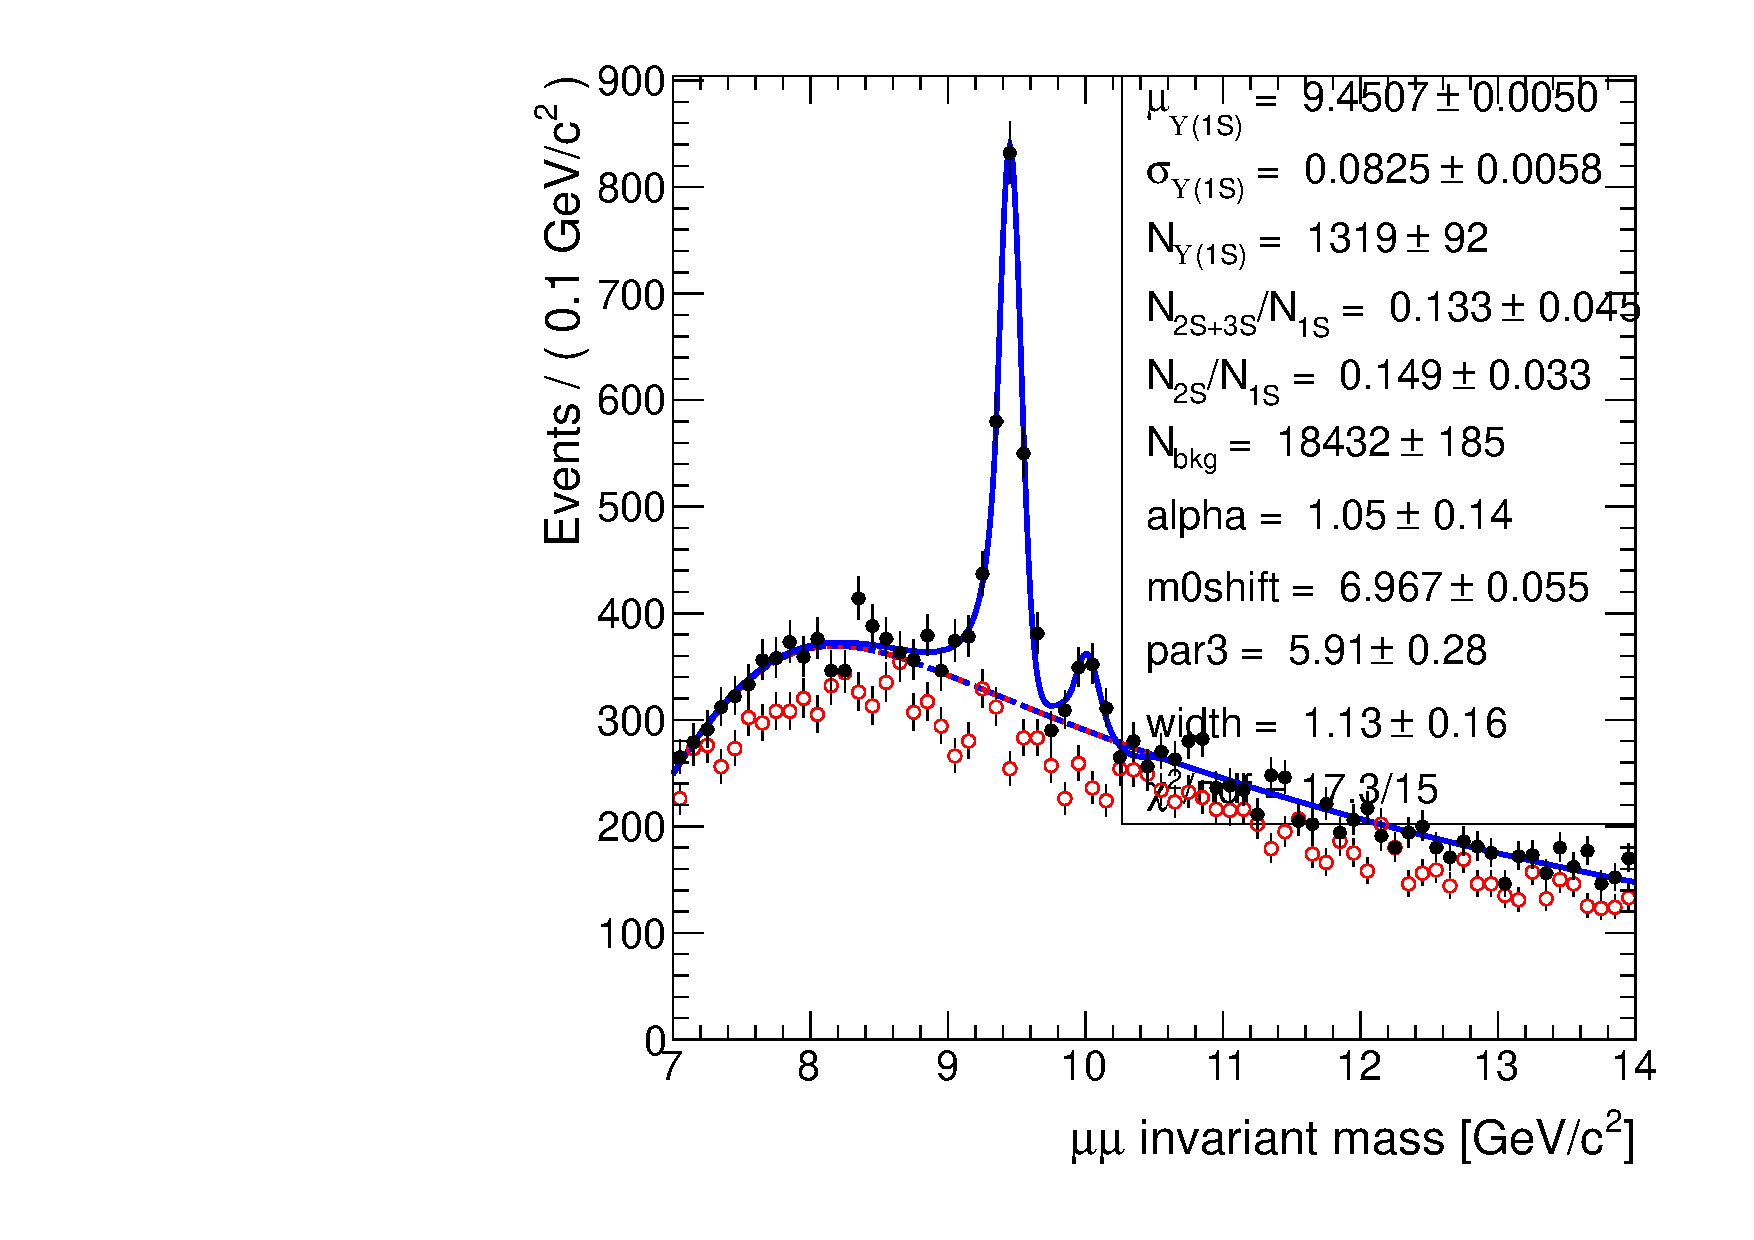
\includegraphics[angle=0,width=0.5\textwidth]{figures/fitting/masspeak_Hi_paramOn_MuonPT35_95imub}}
%  \caption{Mass fit to the  $95 \mu b^{-1}$ dataset.}
%  \label{fig:masfit_95imub}
%  \end{center}
%\end{figure}
%
\begin{figure}[hbtp]
  \begin{center}
    $~$\vspace*{-4mm}
    \subfigure[Minimum bias]{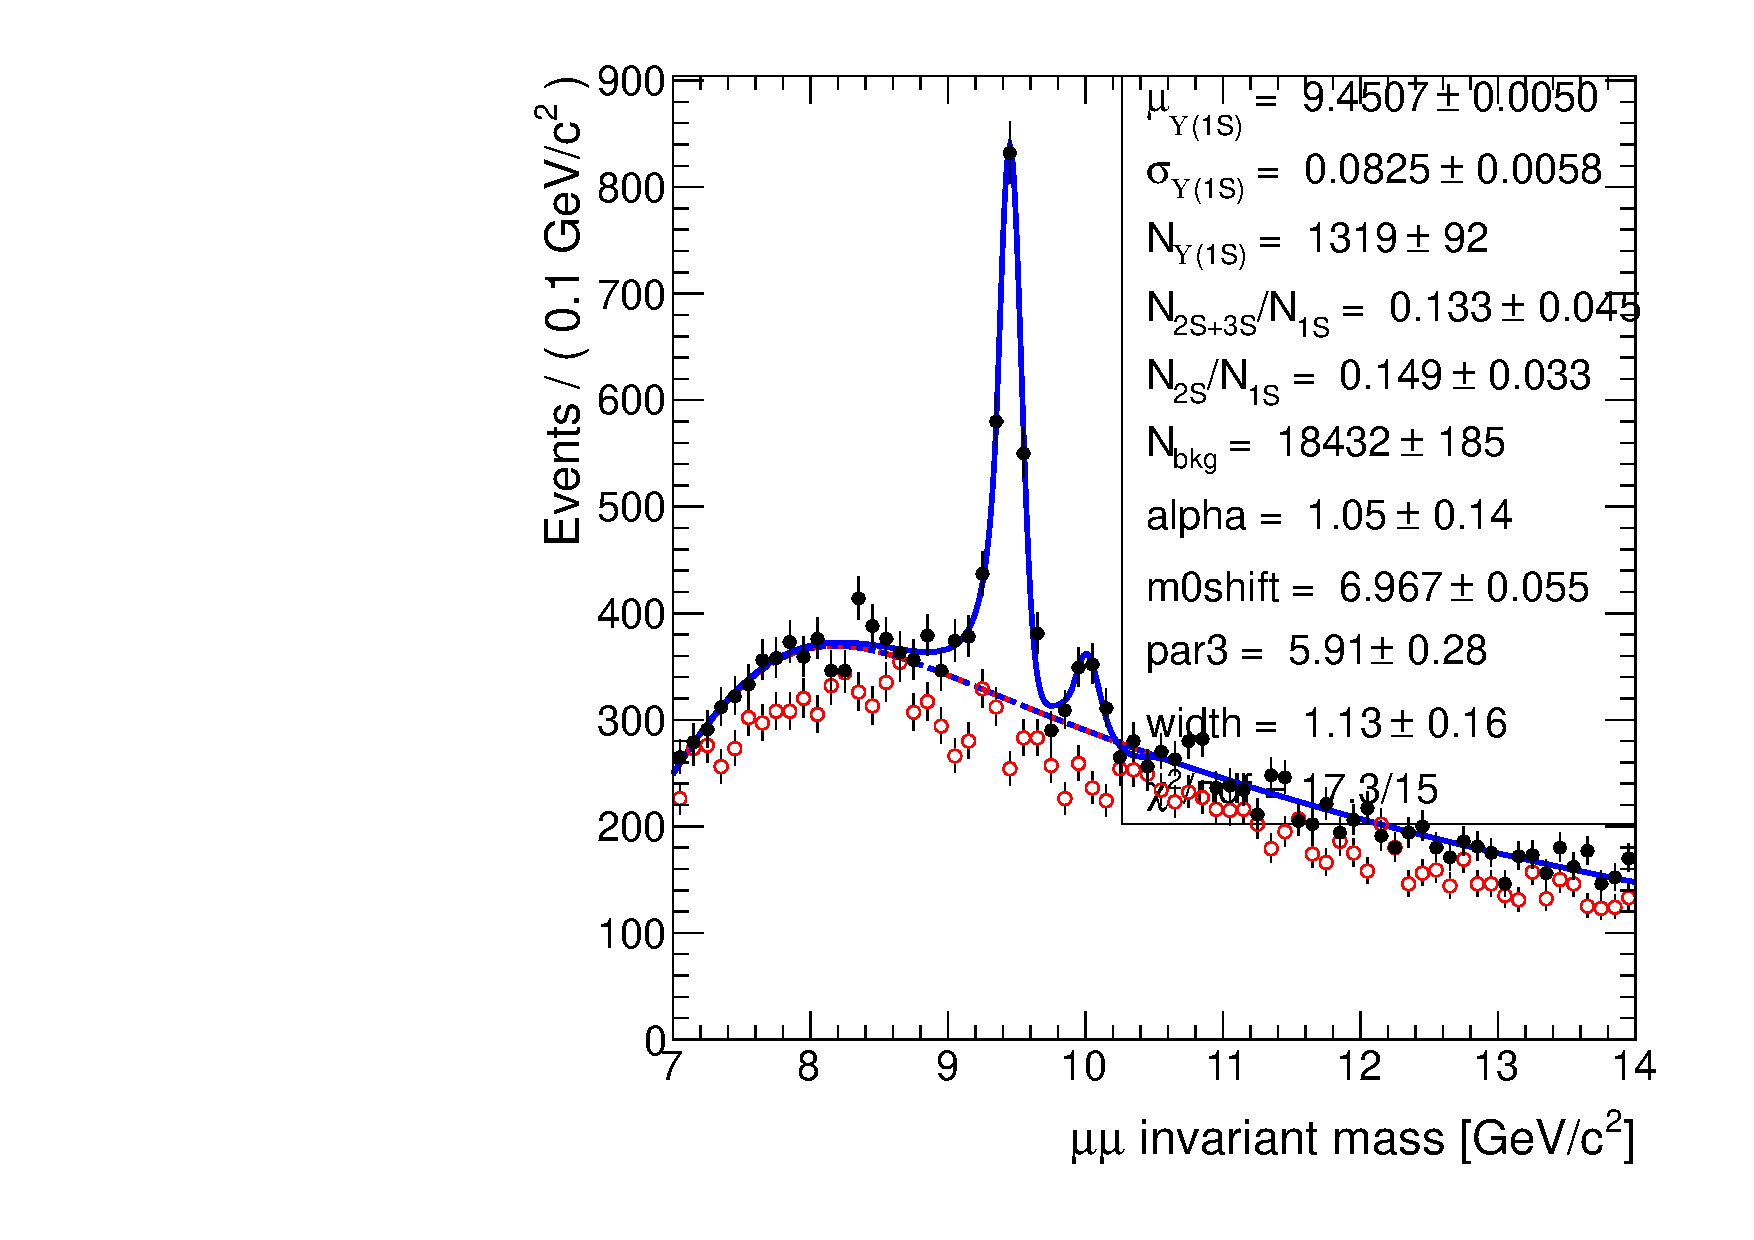
\includegraphics[angle=0,width=0.35\textwidth]{figures/fitting/masspeak_Hi_paramOn_MuonPT35_95imub}}
    \subfigure[Single ratio $R_{23}$ vs centrality (stat. error only)]{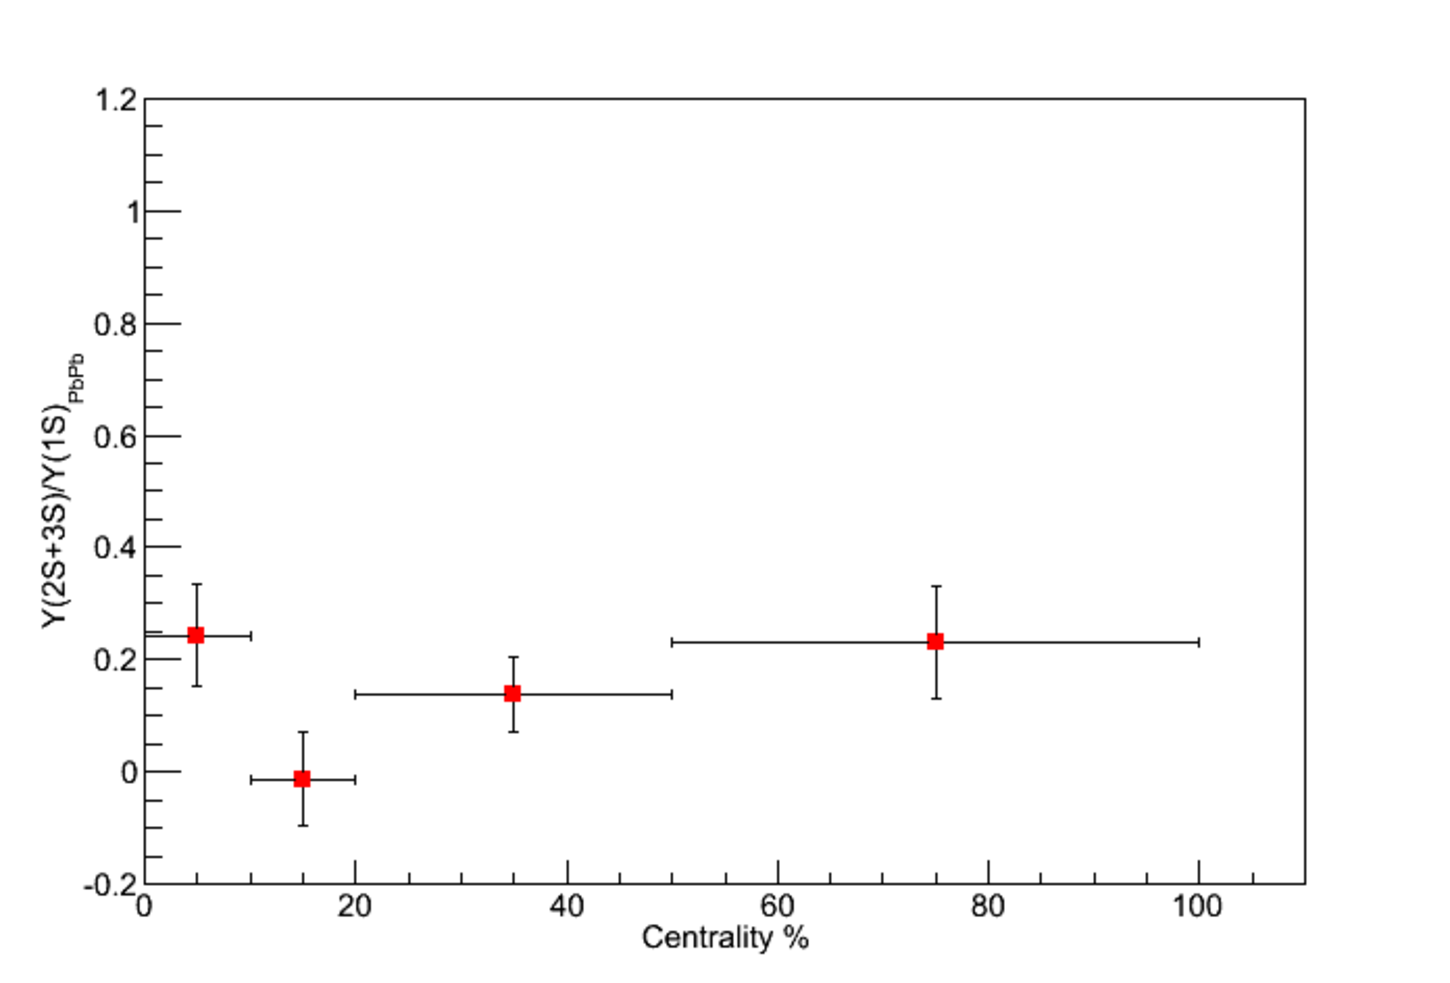
\includegraphics[angle=0,width=0.55\textwidth]{figures/centrality/RatioVsCent_95imub}} \\
    $~$\vspace*{-4mm}
    \subfigure[ 0- 10\%]{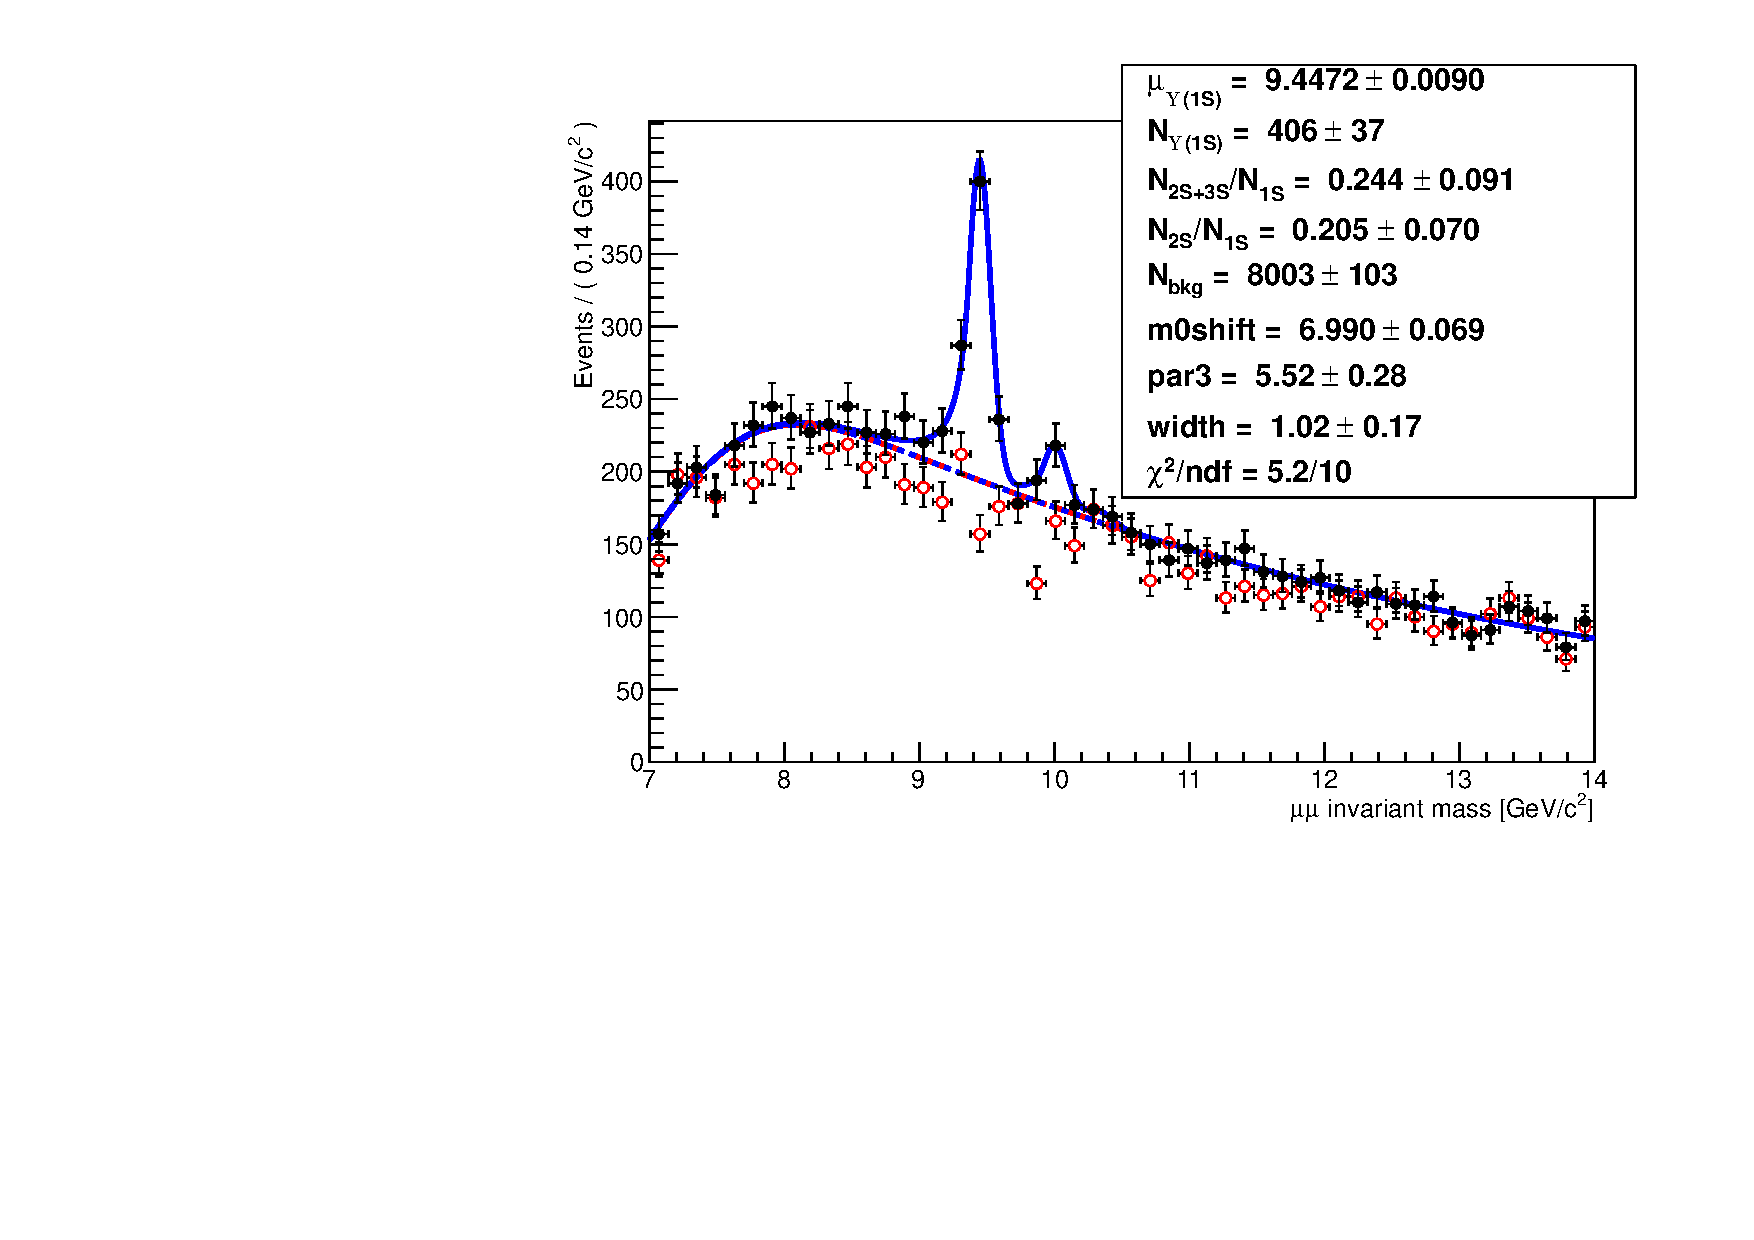
\includegraphics[angle=0,width=0.42\textwidth]{figures/centrality/masspeak_Hi_paramOn_cntr0-10_pt35_95imub}}
    \subfigure[10- 20\%]{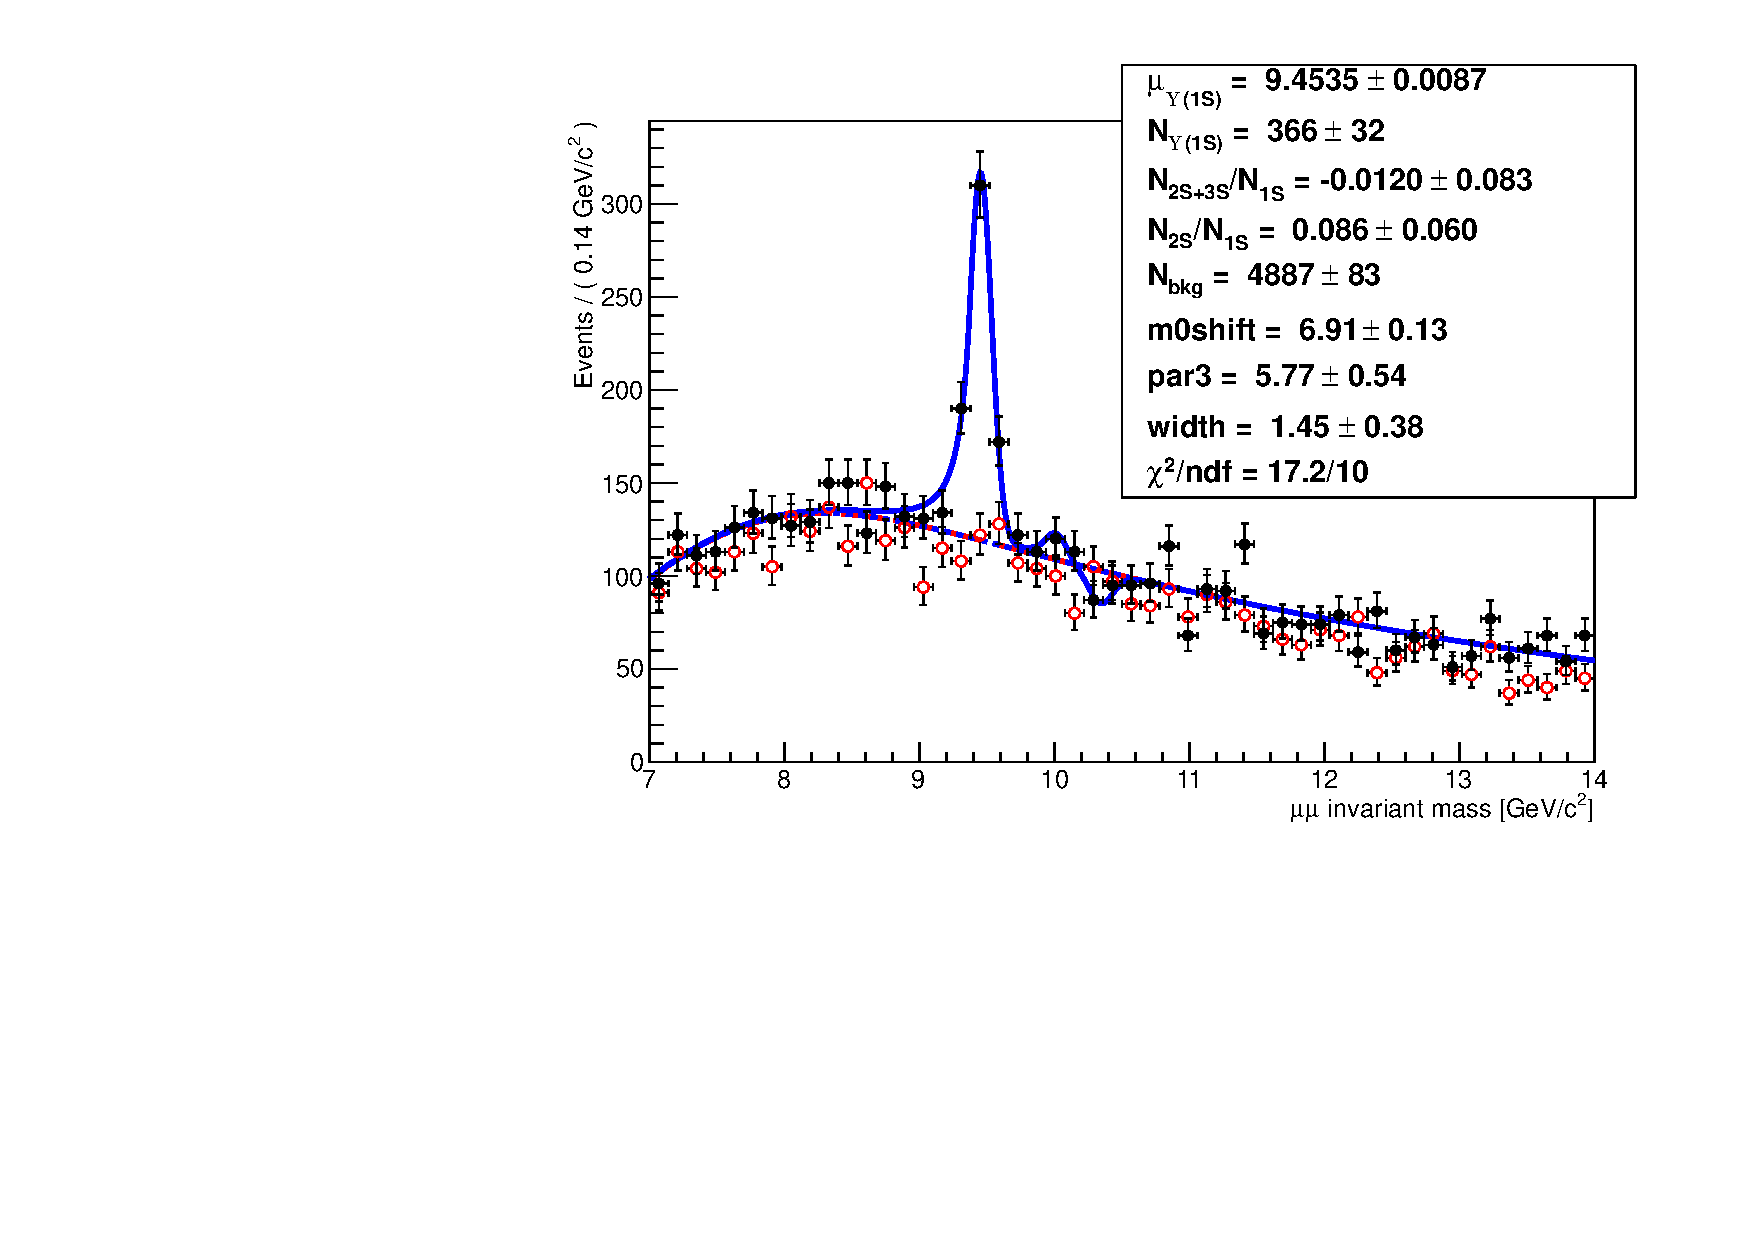
\includegraphics[angle=0,width=0.42\textwidth]{figures/centrality/masspeak_Hi_paramOn_cntr10-20_pt35_95imub}}\\
    \subfigure[20- 50\%]{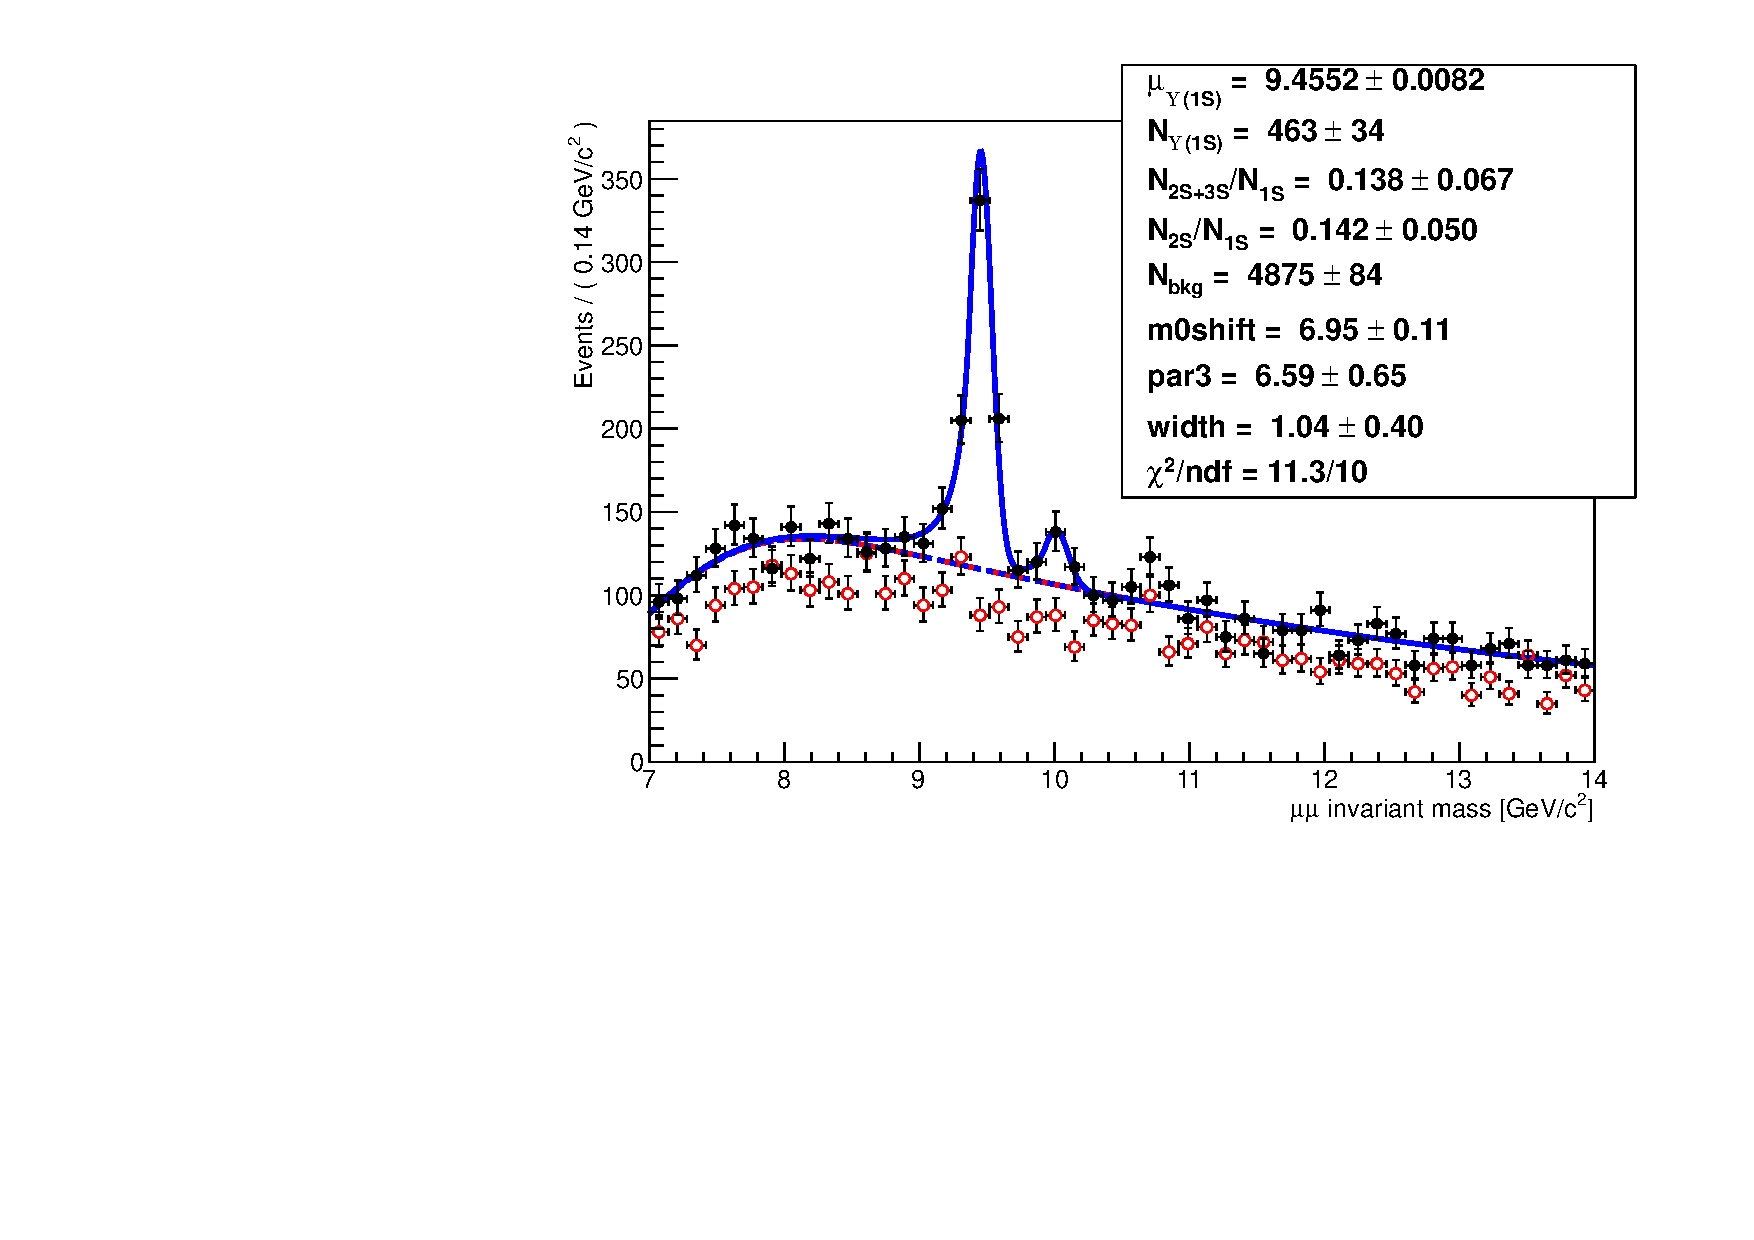
\includegraphics[angle=0,width=0.42\textwidth]{figures/centrality/masspeak_Hi_paramOn_cntr20-50_pt35_95imub}}
    \subfigure[50-100\%]{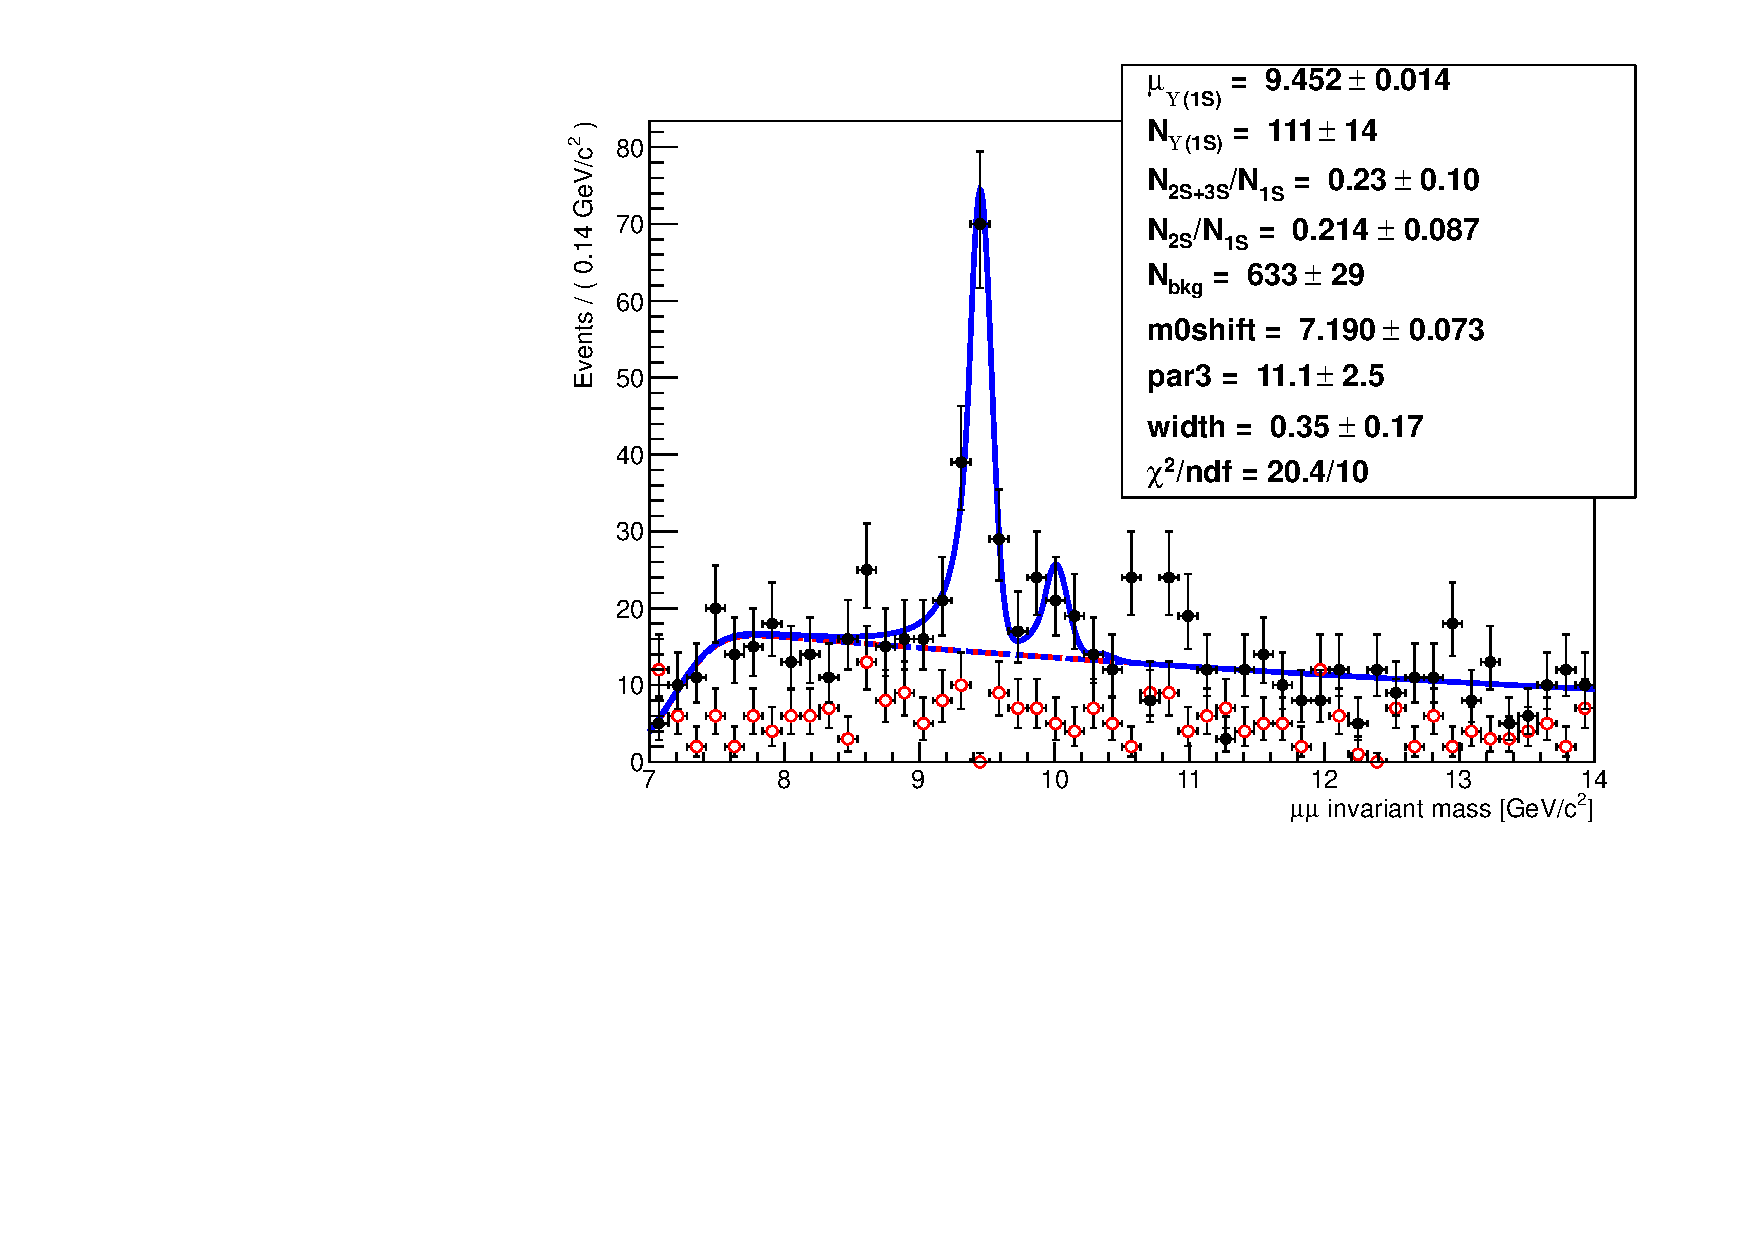
\includegraphics[angle=0,width=0.42\textwidth]{figures/centrality/masspeak_Hi_paramOn_cntr50-100_pt35_95imub}}\\
    \caption{Results from the   $95 \mu b^{-1}$ dataset. ($\pt>3.5\GeVc$)}
  \label{fig:massfit_singlerat_centrality_95imub}
  \end{center}
\end{figure}

%\begin{figure}[hbtp]
%  \begin{center}
%    \caption{Centrality dependence of the single ratio; only the statistical uncertainty is included.}
%    \label{fig:massfit_singlerat_centrality_95imub}
%  \end{center}
%\end{figure}

%\clearpage
%
%%NOTE: following section has incorrect results, based on duplicated data ttree
%\subsection{Results with $150 \mu b^{-1}$}
%\label{sec:newdata150}
%
%\begin{figure}[hbtp]
%  \begin{center}
%  %\subfigure[$\chi_{23}$]
%    \subfigure[$pt^\mu>3.5\GeVc$]{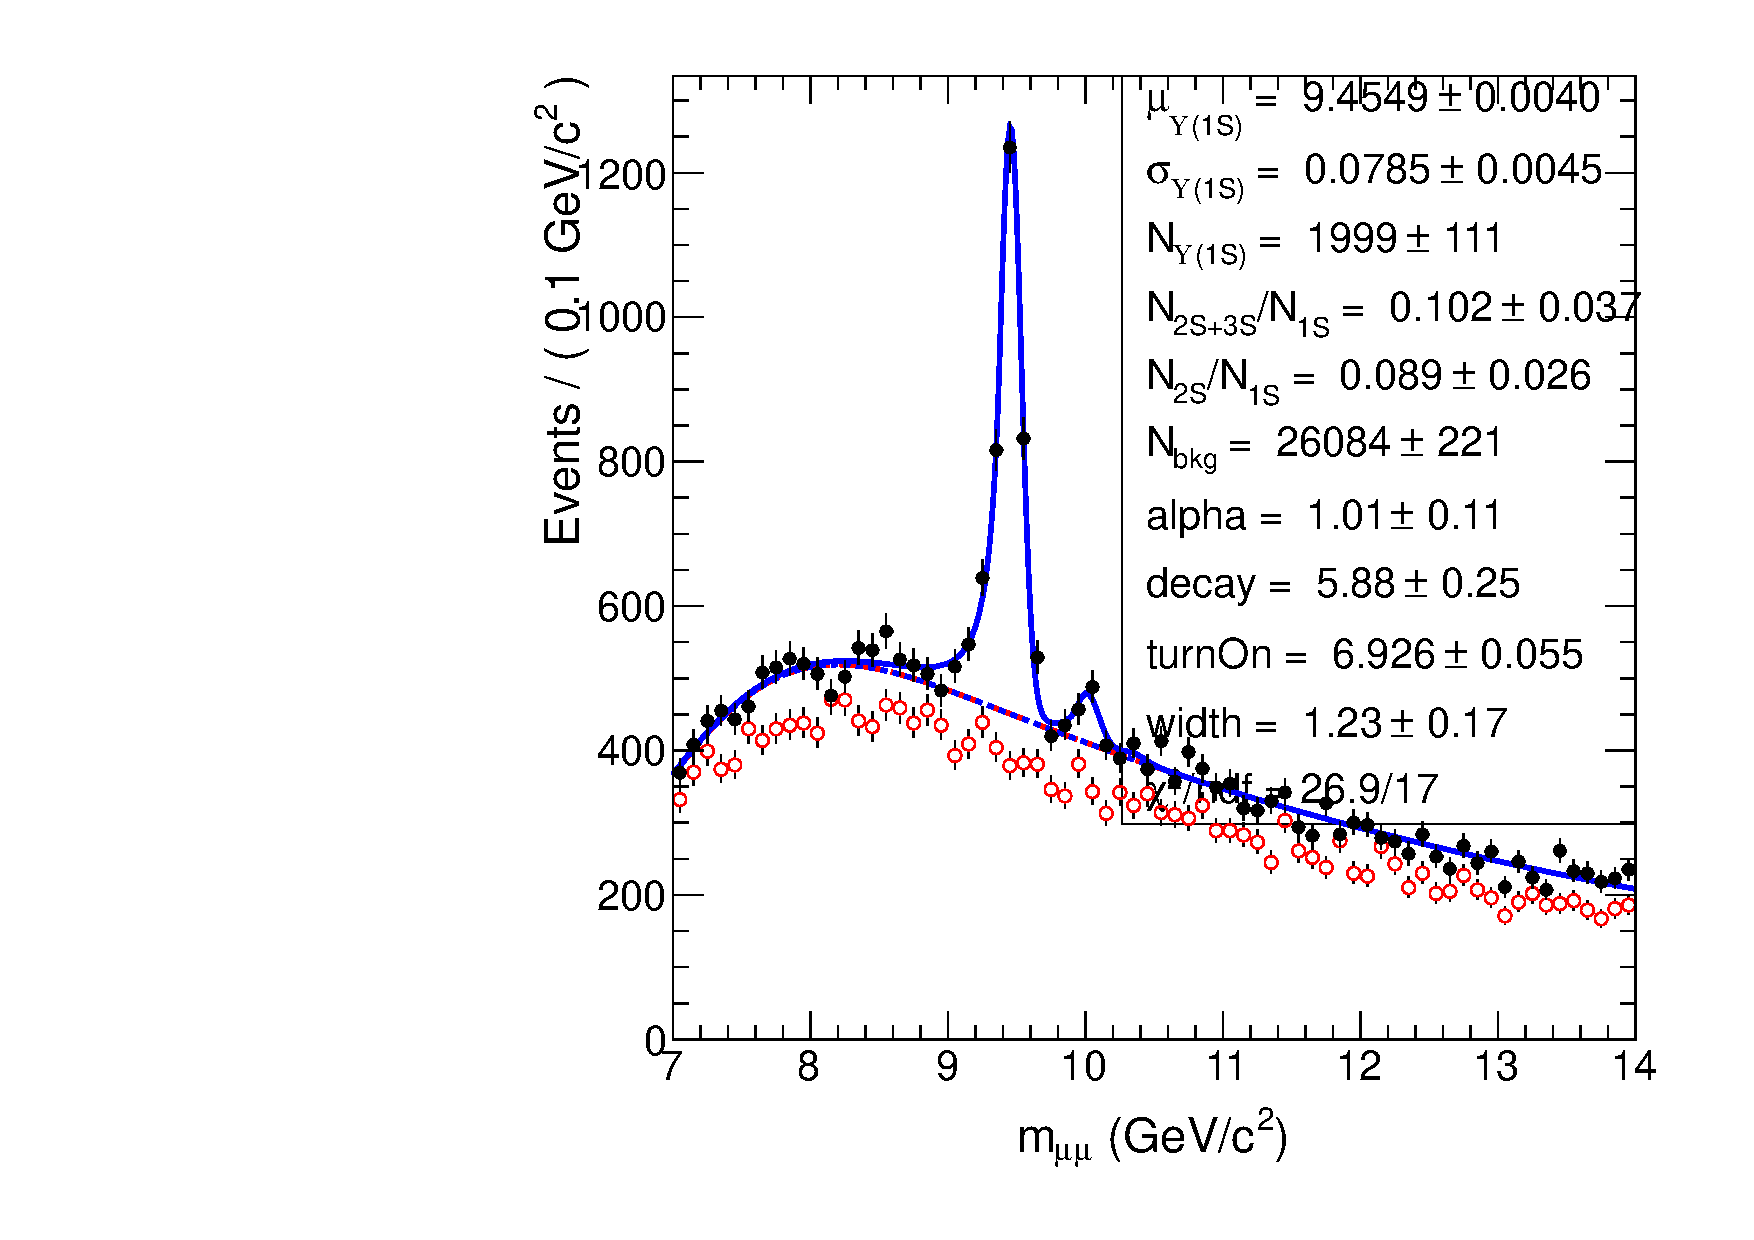
\includegraphics[angle=0,width=0.5\textwidth]{figures/fitting/masspeak_Hi_paramOn_MuonPT35_150imub}}
%    \subfigure[$pt^\mu>4.0\GeVc$]{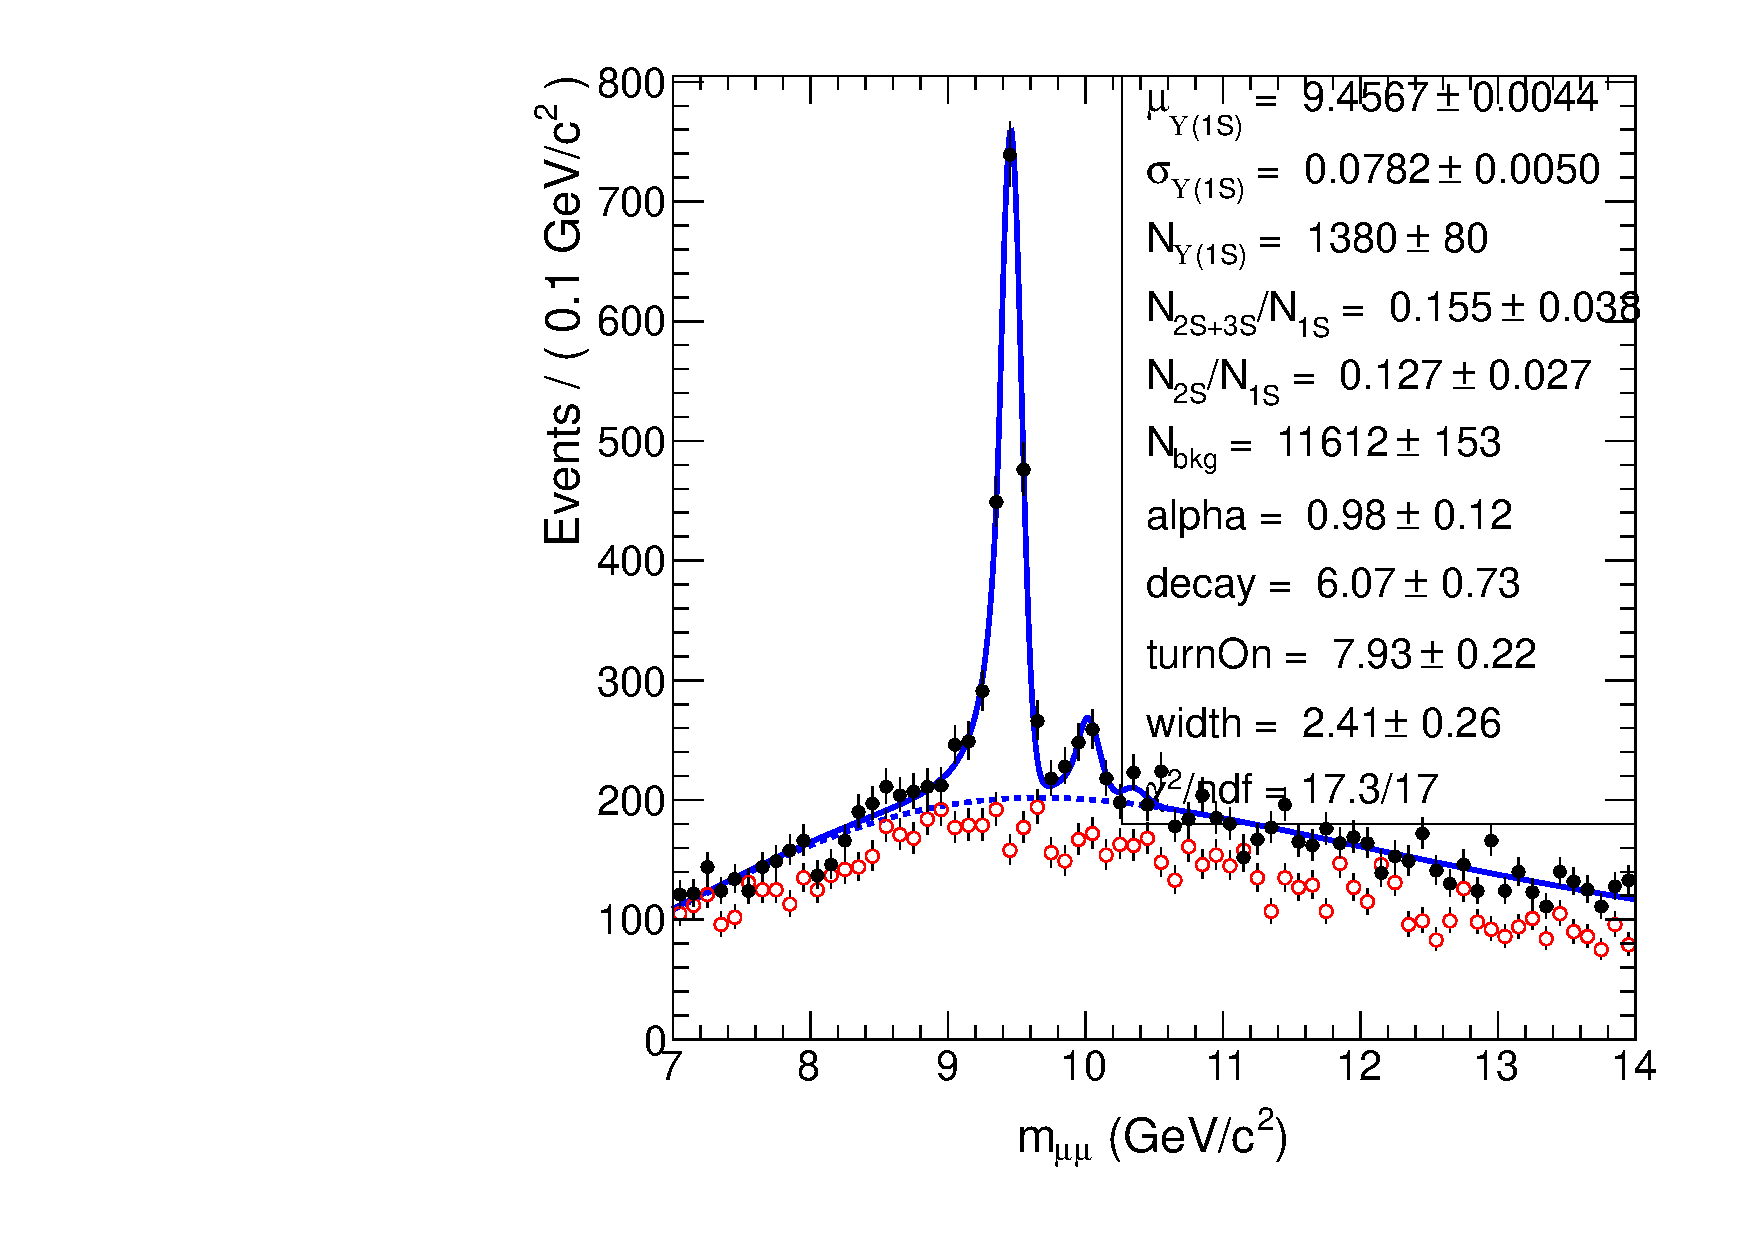
\includegraphics[angle=0,width=0.5\textwidth]{figures/fitting/masspeak_Hi_paramOn_MuonPT4_150imub}}
%    \caption{Nominal mass fits to the  $150 \mu b^{-1}$ dataset.}
%    \label{fig:masfit_150imub}
%  \end{center}
%\end{figure}
%
%
%\begin{figure}[hbtp]
%  \begin{center}
%\subfigure[ 0- 10\%]{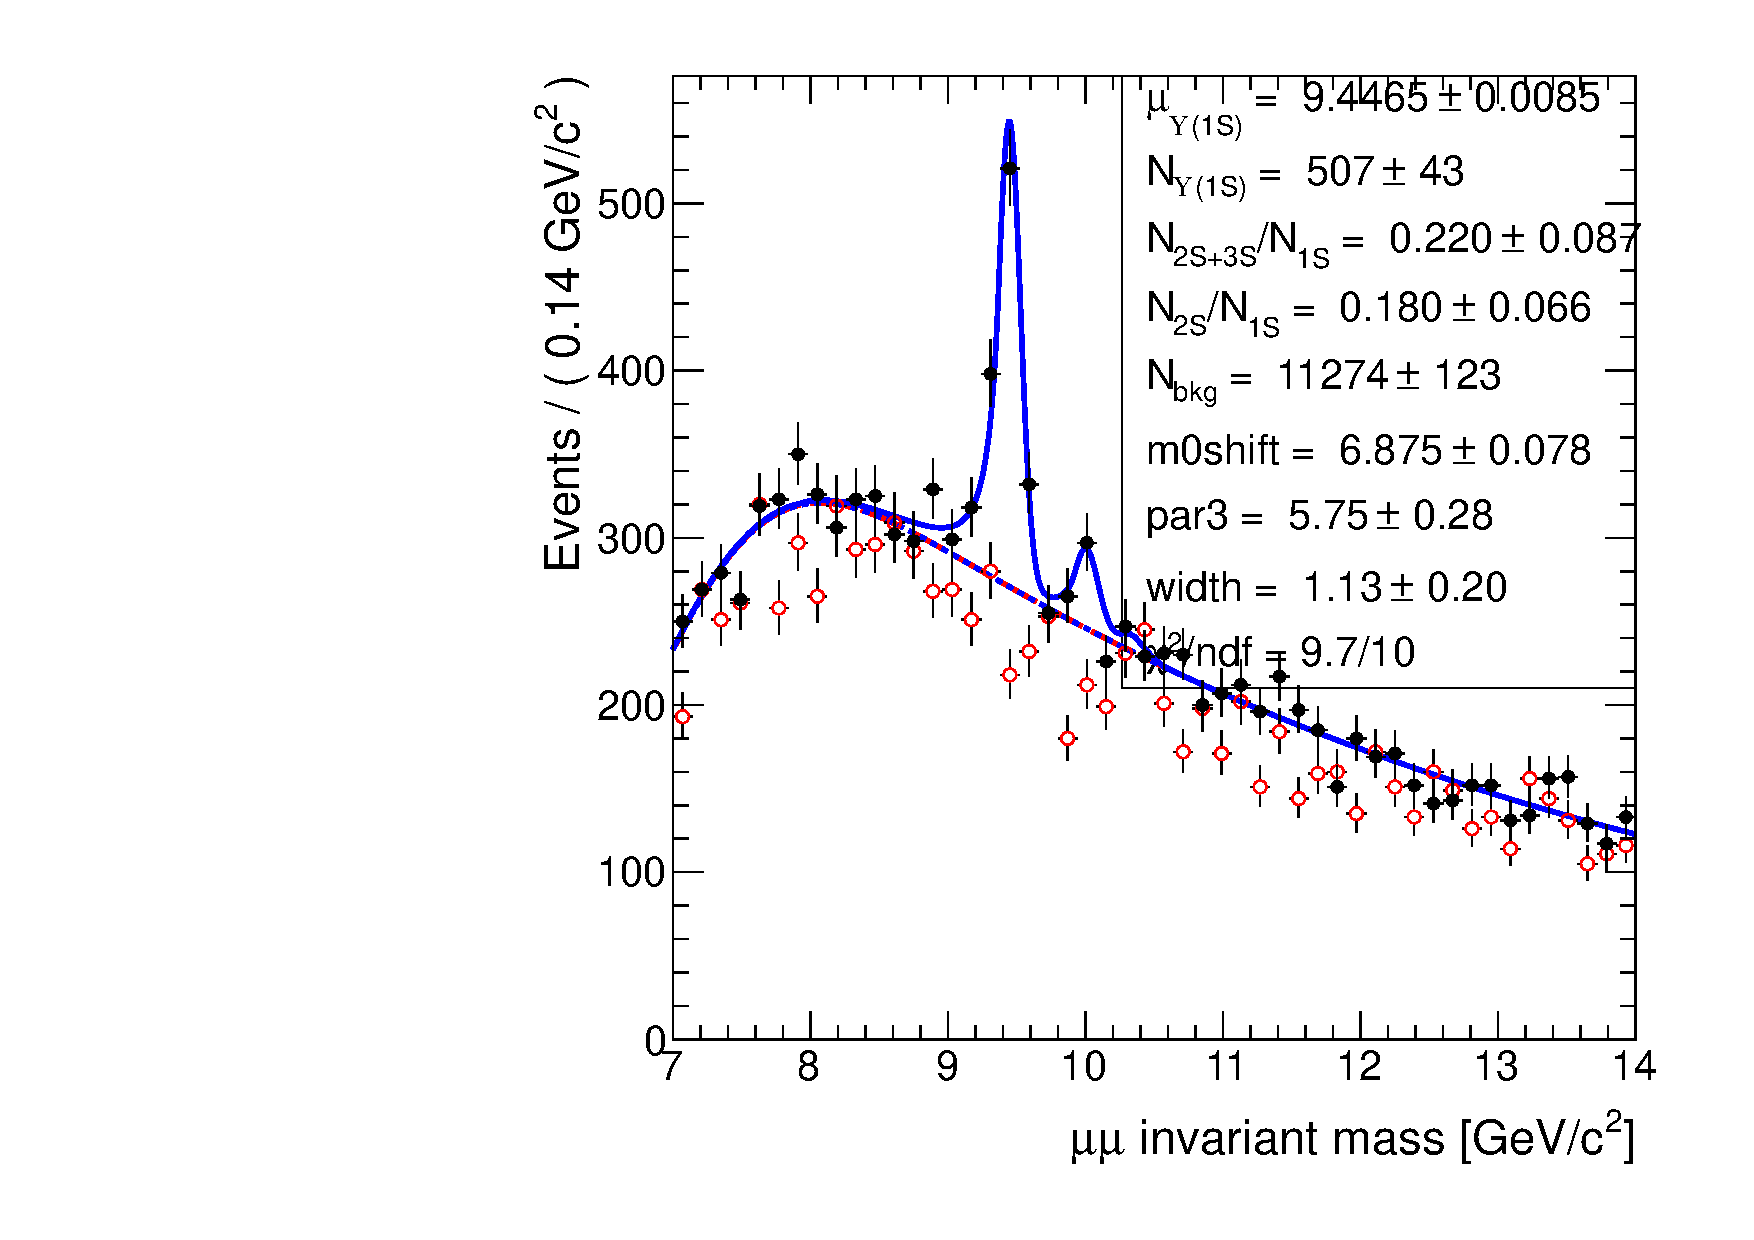
\includegraphics[angle=0,width=0.45\textwidth]{figures/centrality/masspeak_Hi_paramOn_cntr0-10_pt35_150imub}}
%\subfigure[10- 20\%]{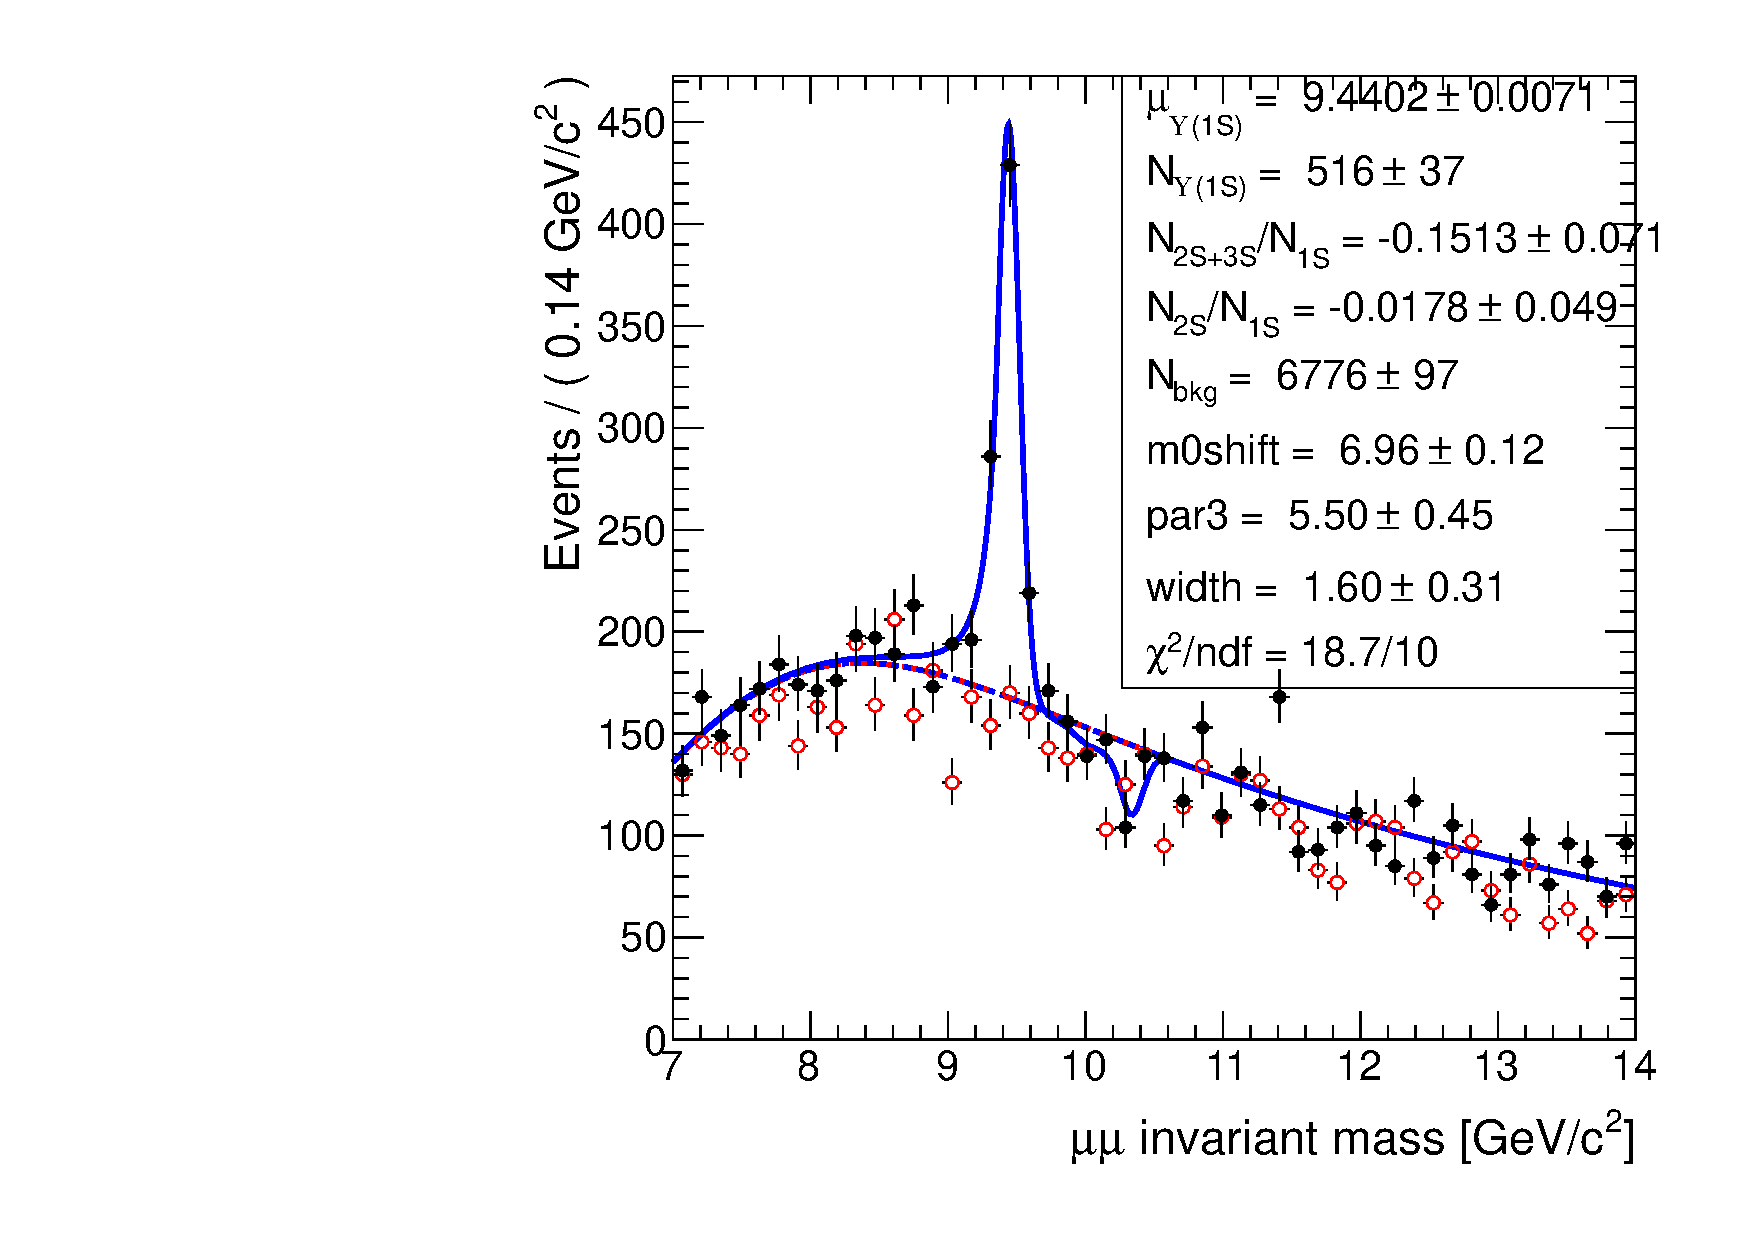
\includegraphics[angle=0,width=0.45\textwidth]{figures/centrality/masspeak_Hi_paramOn_cntr10-20_pt35_150imub}}\\
%\subfigure[20- 50\%]{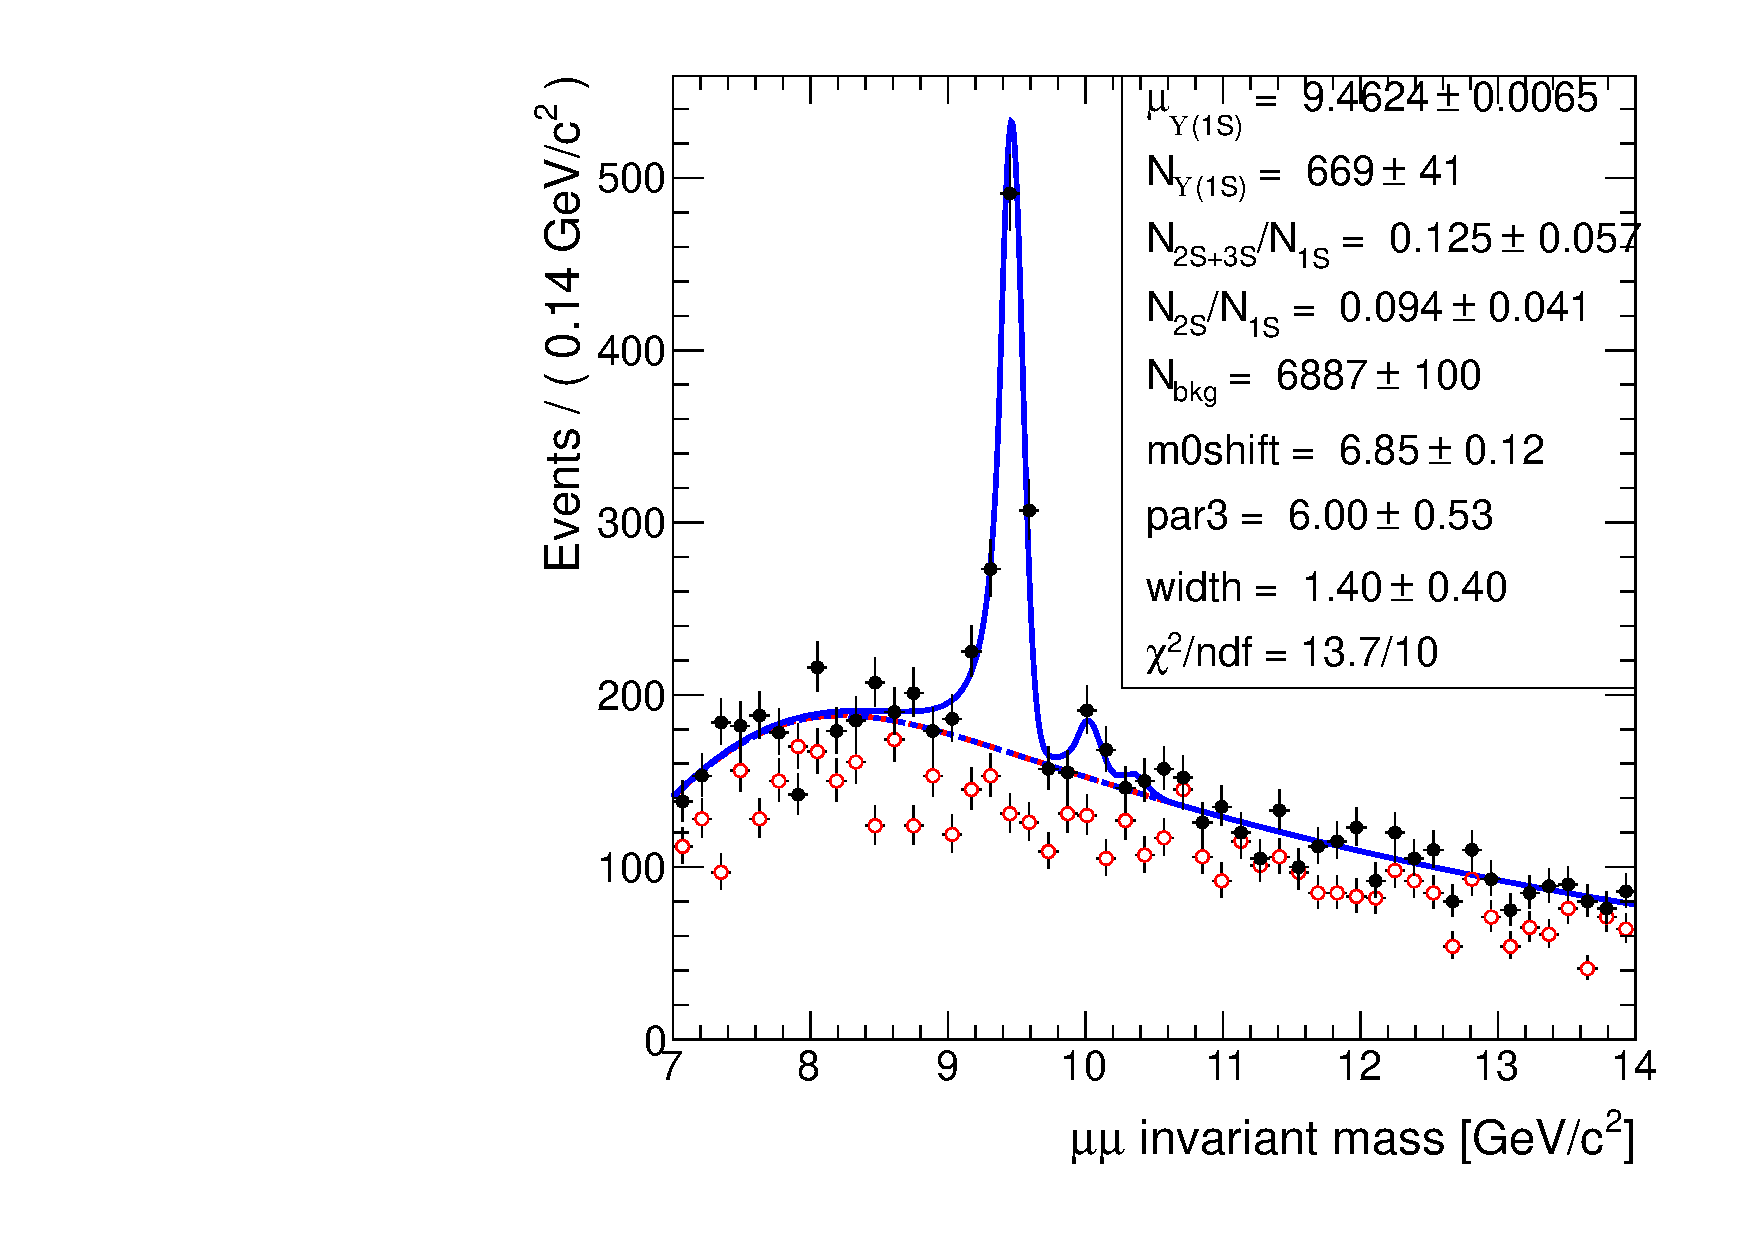
\includegraphics[angle=0,width=0.45\textwidth]{figures/centrality/masspeak_Hi_paramOn_cntr20-50_pt35_150imub}}
%\subfigure[50-100\%]{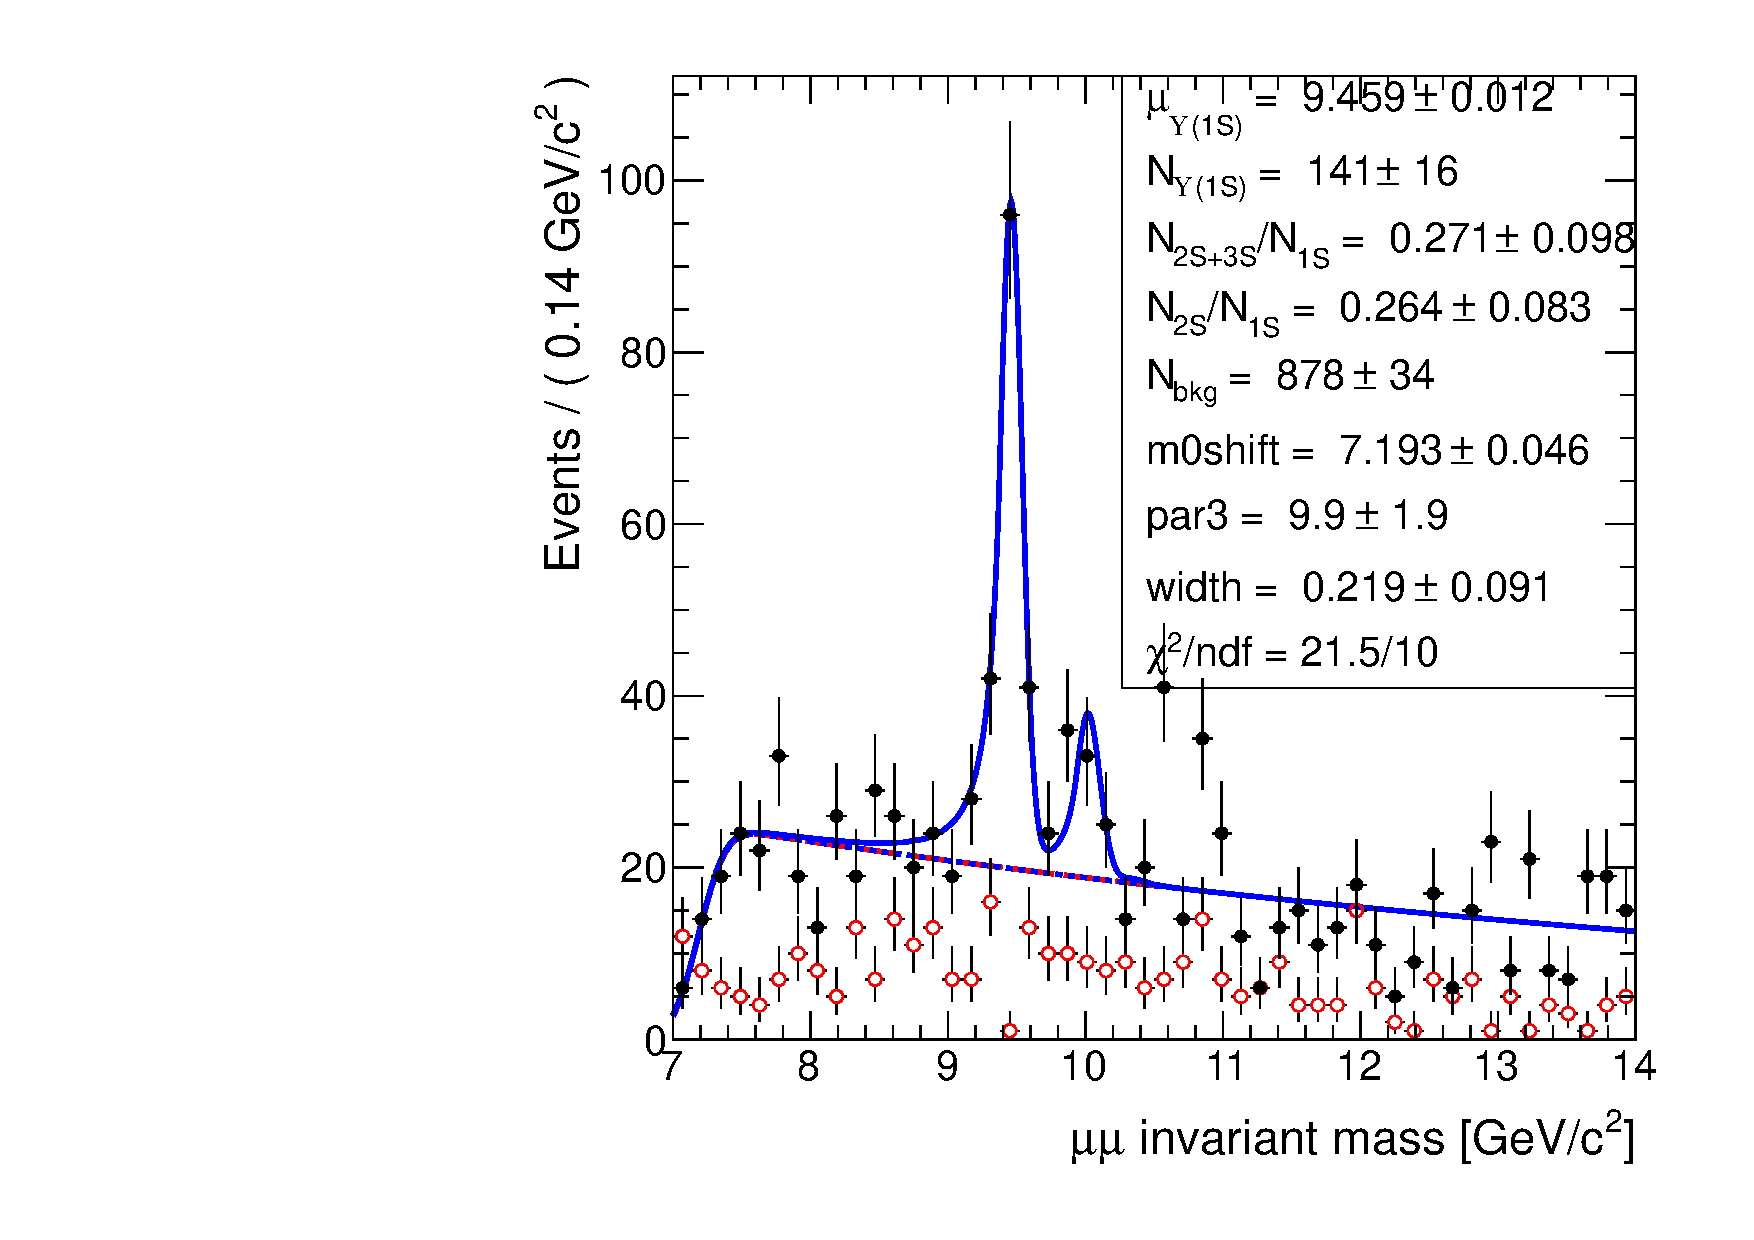
\includegraphics[angle=0,width=0.45\textwidth]{figures/centrality/masspeak_Hi_paramOn_cntr50-100_pt35_150imub}}\\
%\subfigure[Double ratio $\chi_{2}$ vs centrality]{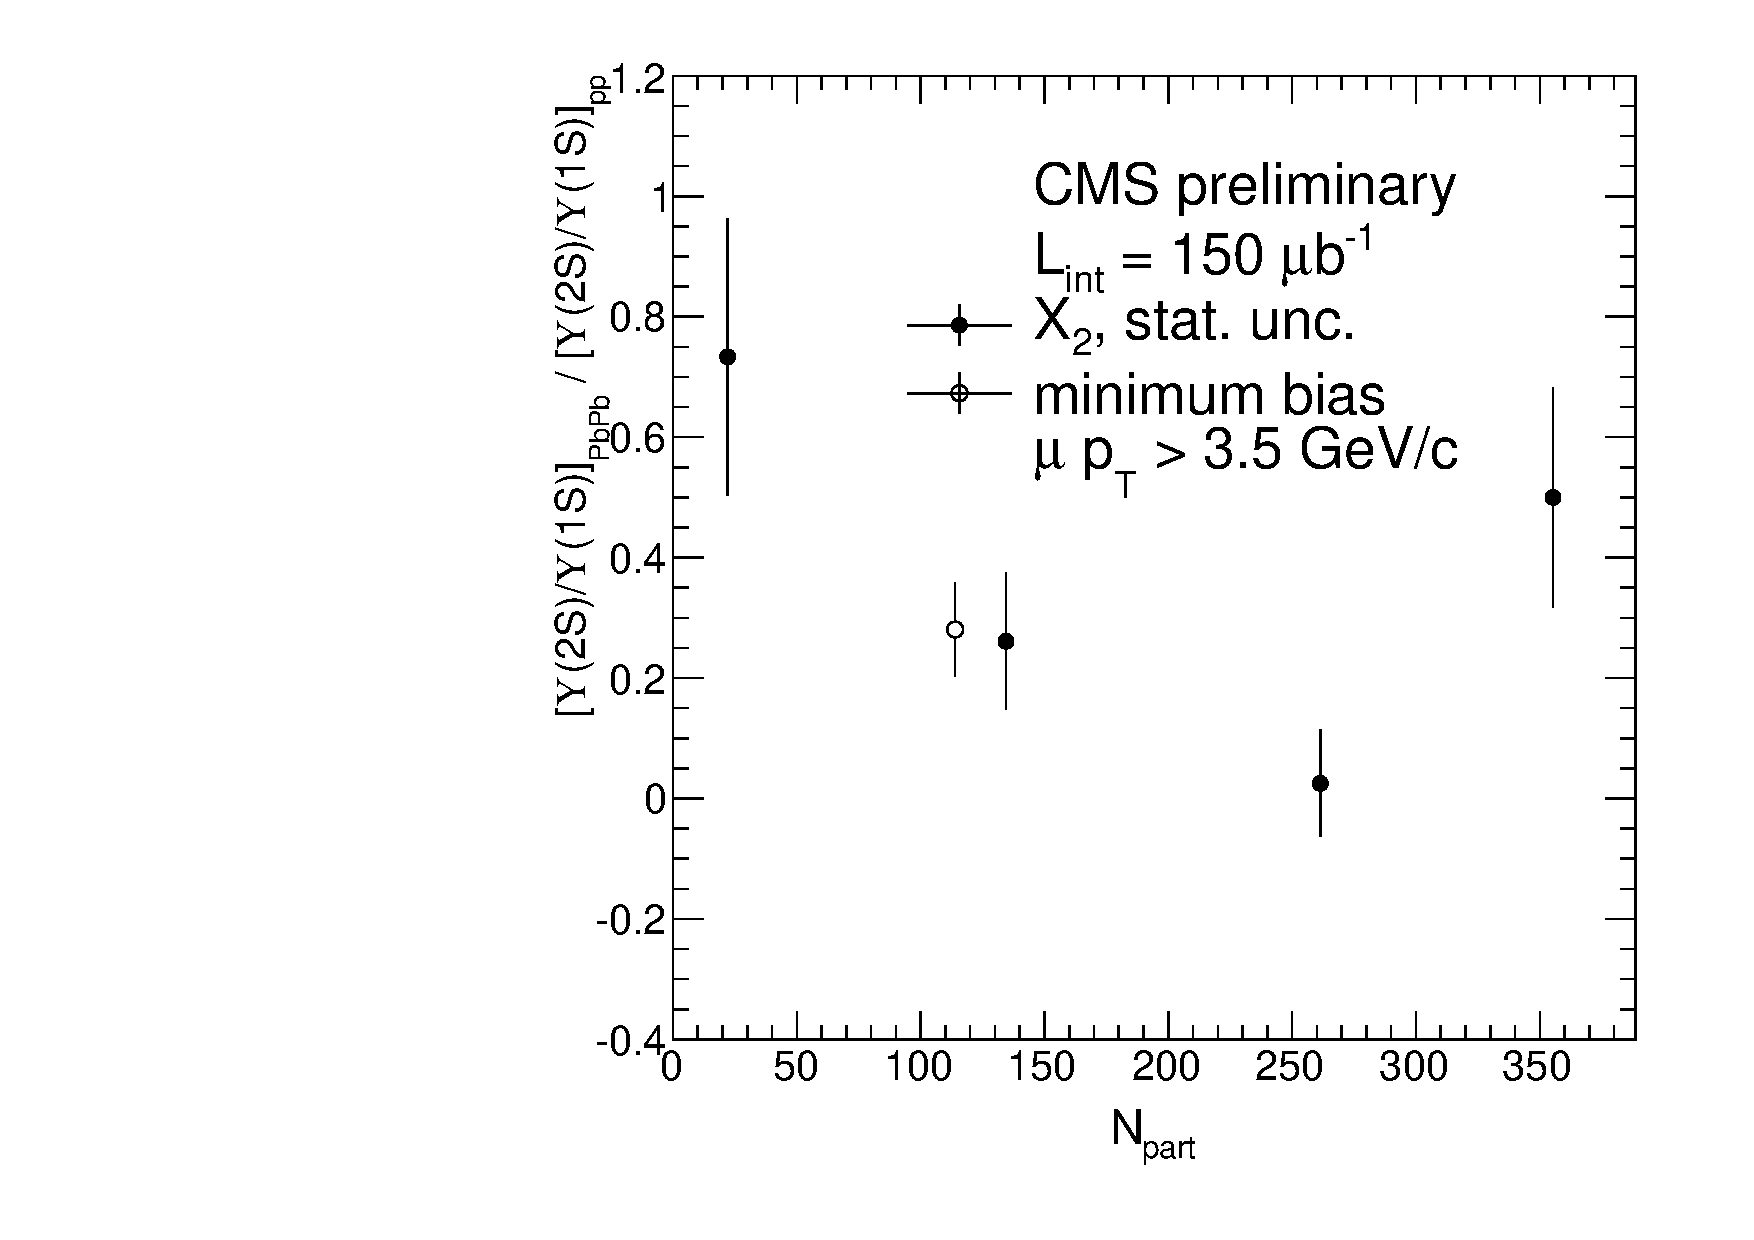
\includegraphics[angle=0,width=0.45\textwidth]{figures/centrality/chi2pt35}} 
%\subfigure[Double ratio $\chi_{23}$ vs centrality]{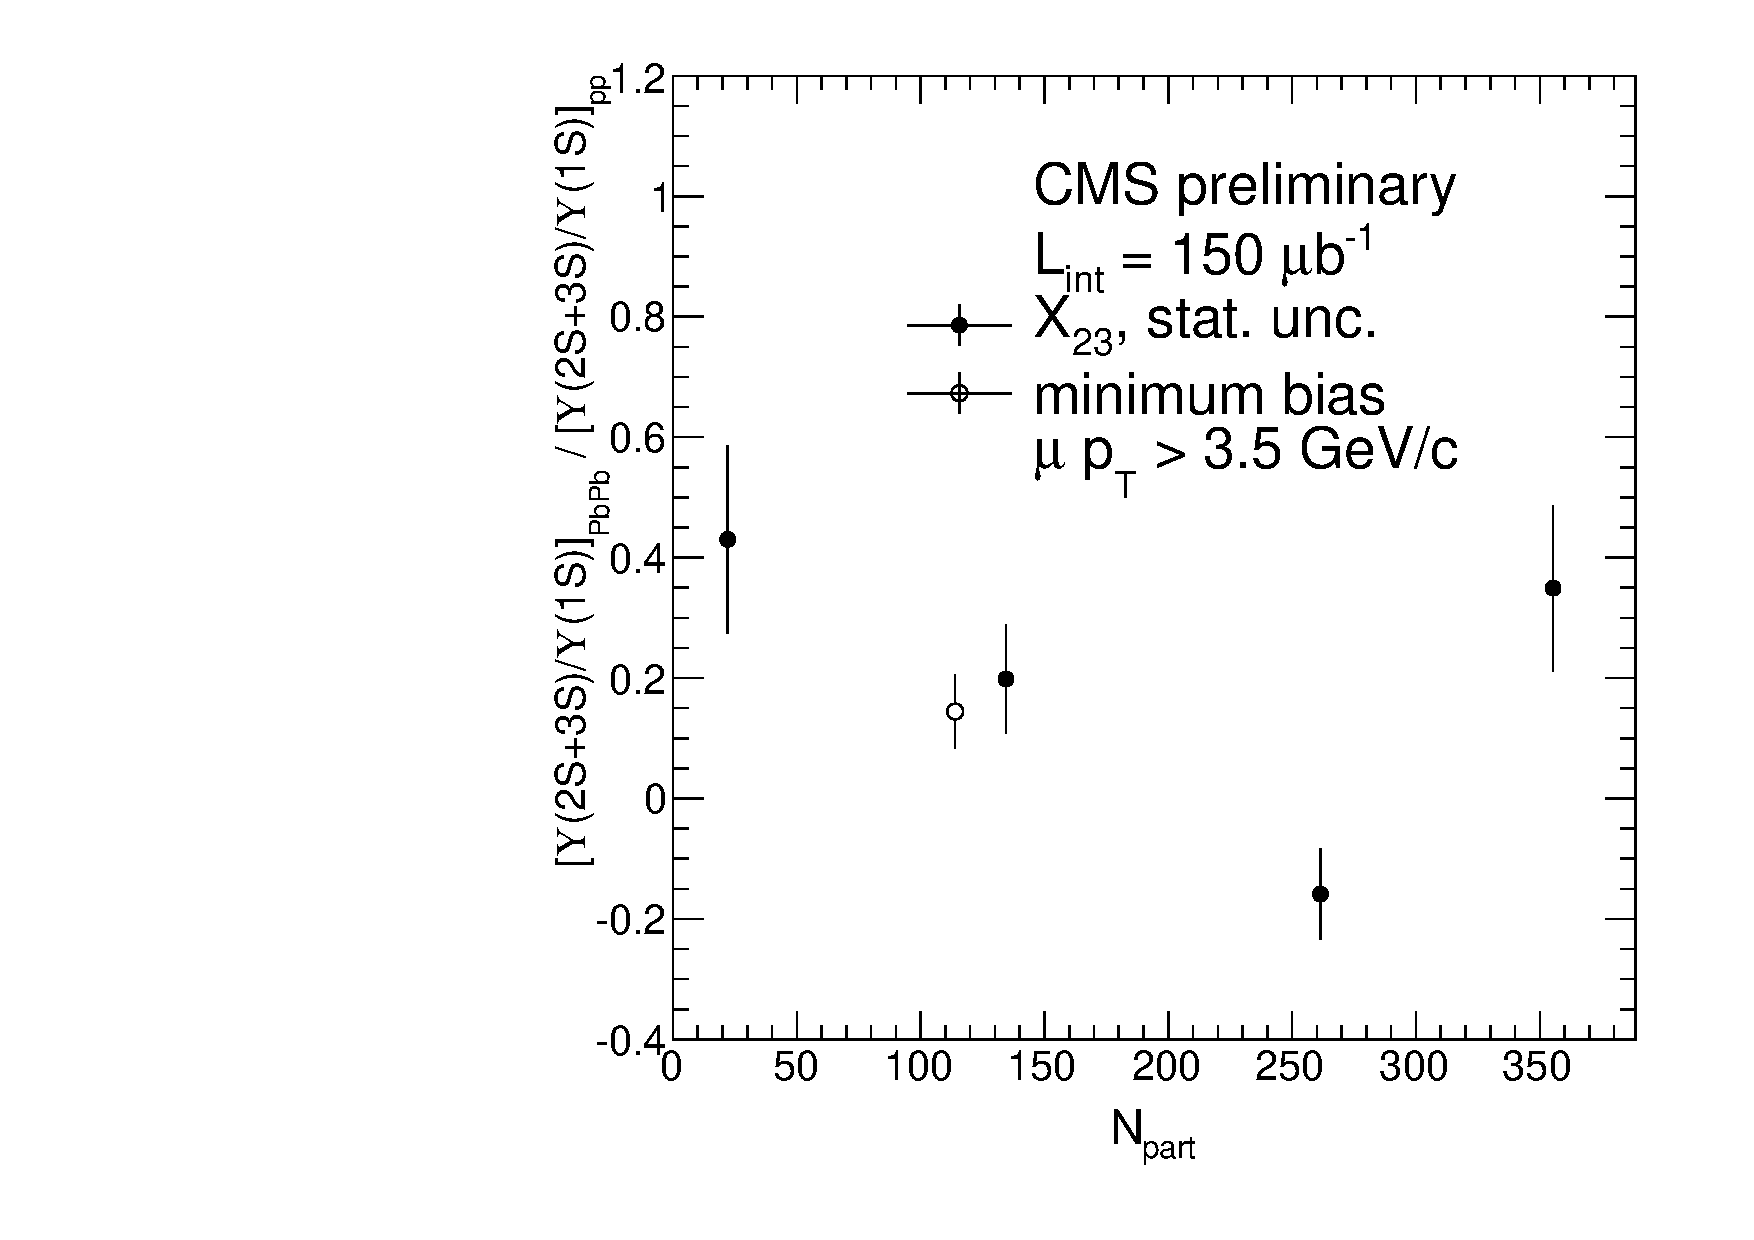
\includegraphics[angle=0,width=0.45\textwidth]{figures/centrality/chi23pt35}} 
%%\subfigure[Single ratio $R_{23}$ vs centrality (stat. error only)]{\includegraphics[angle=0,width=0.55\textwidth]{figures/centrality/RatioVsCent_150imub}} 
%  \caption{Centrality dependent results from the $150 \mu b^{-1}$ dataset. ($\pt>3.5\GeVc$)}
%  \label{fig:massfit_singlerat_centrality_150imub}
%  \end{center}
%\end{figure}
%
%\begin{figure}[hbtp]
%  \begin{center}
%\subfigure[ 0- 10\%]{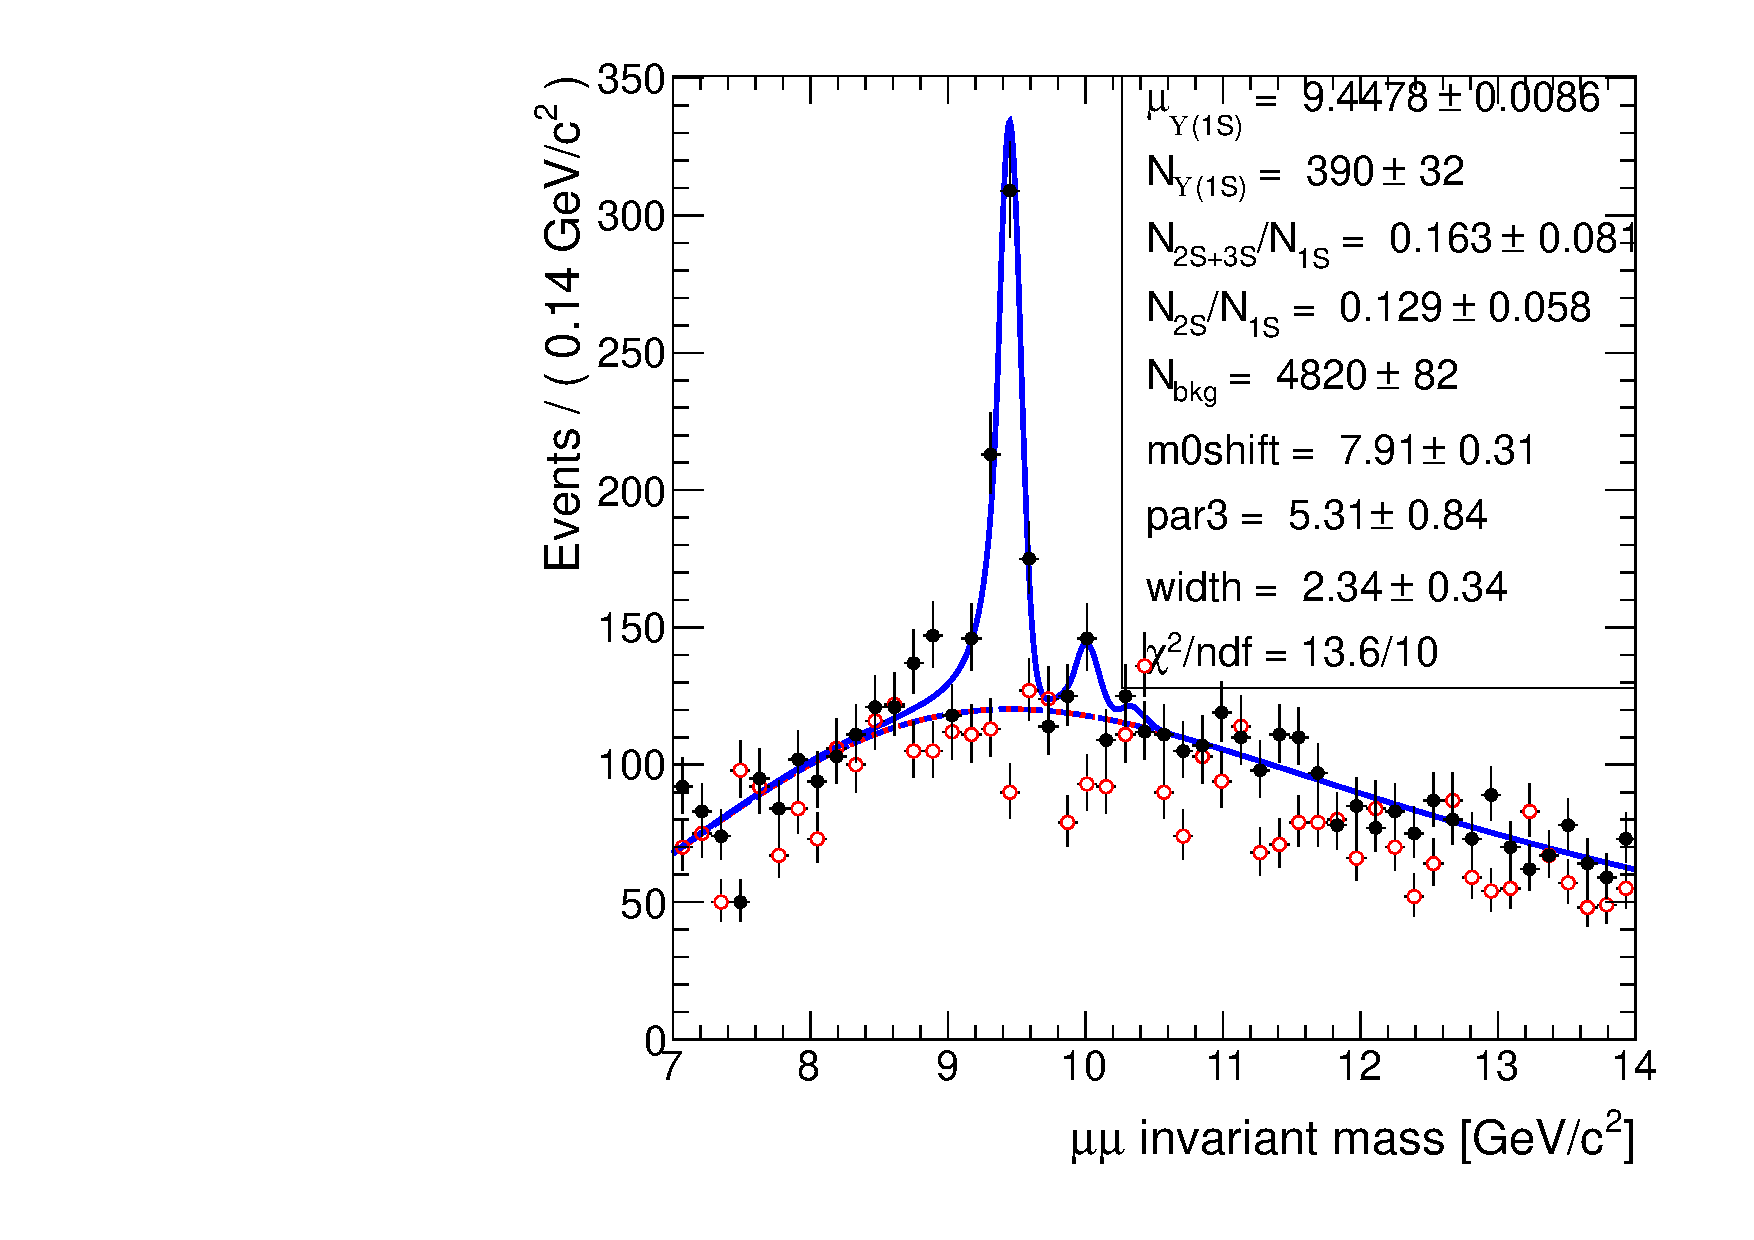
\includegraphics[angle=0,width=0.45\textwidth]{figures/centrality/masspeak_Hi_paramOn_cntr0-10_pt4_150imub}}
%\subfigure[10- 20\%]{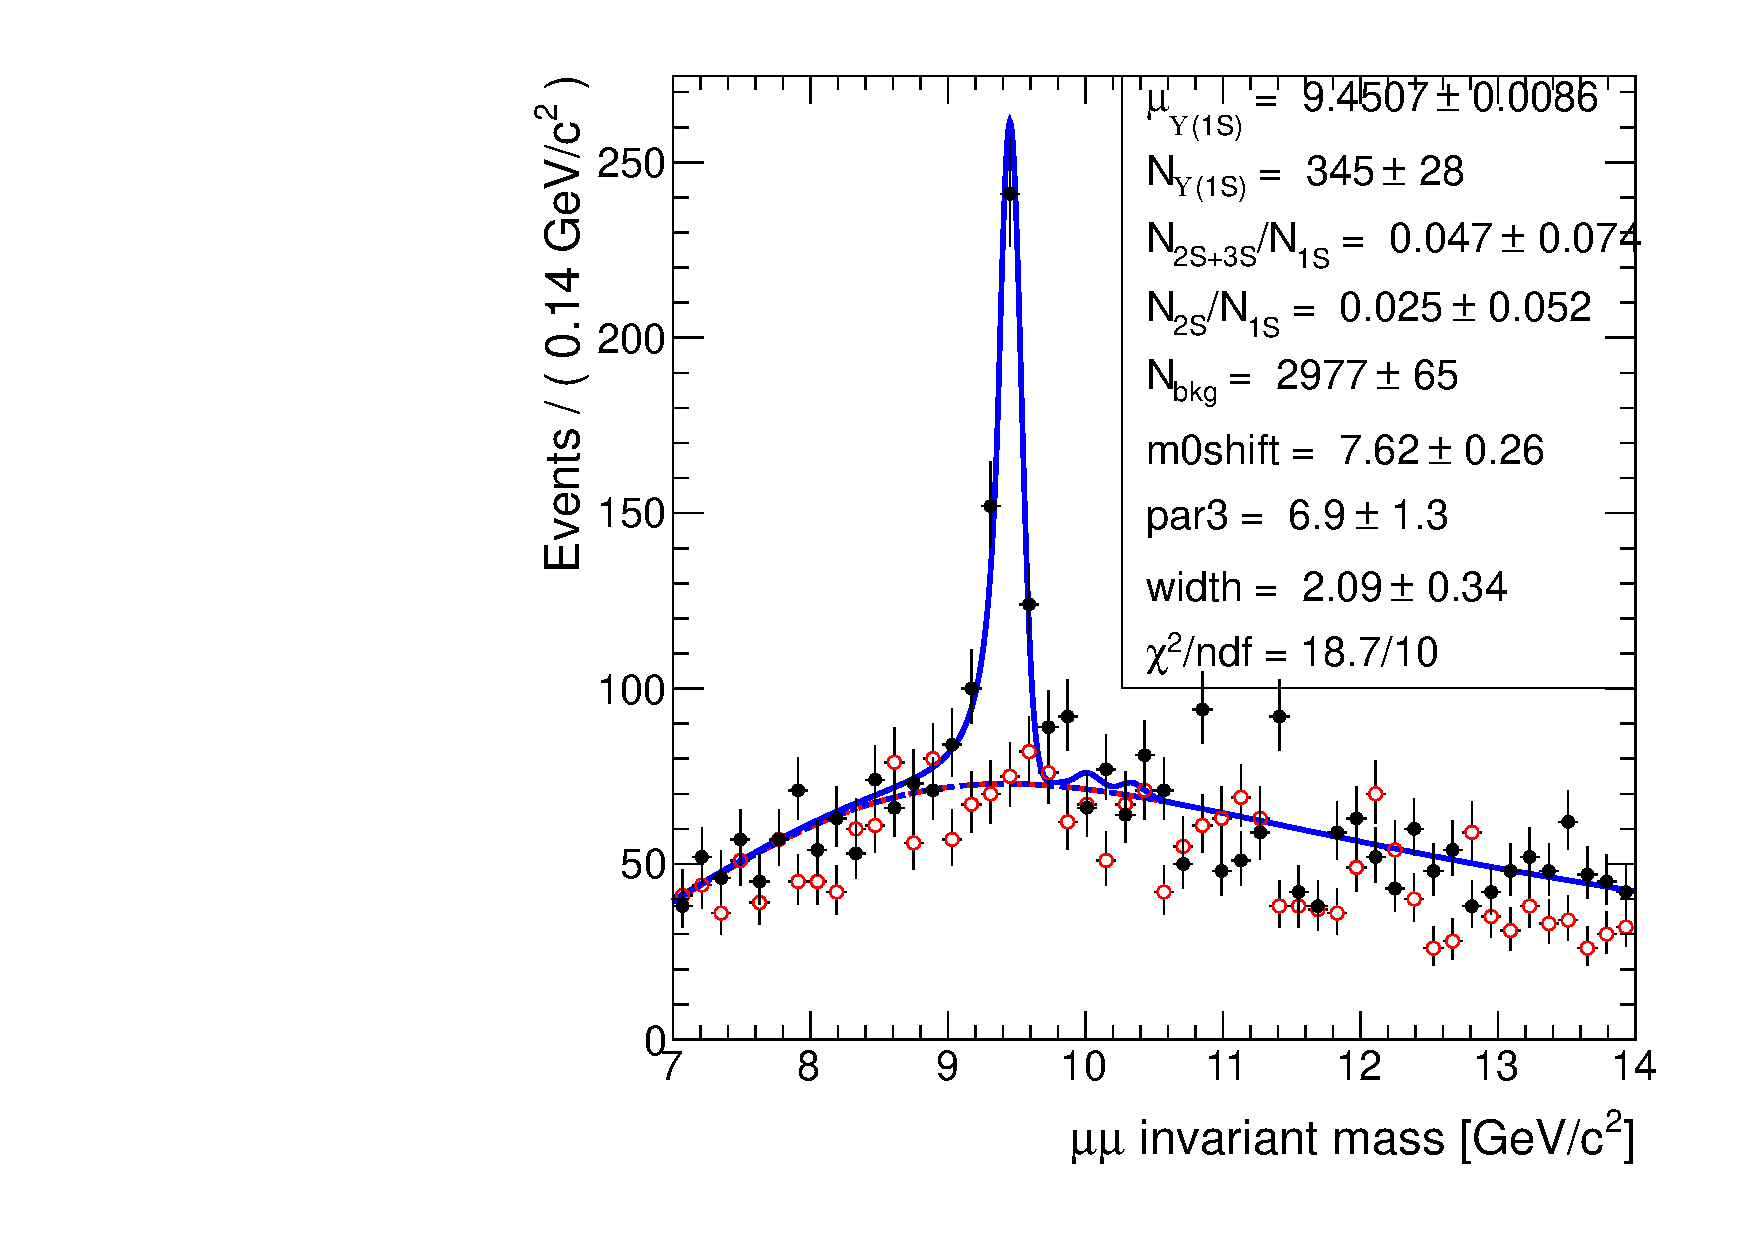
\includegraphics[angle=0,width=0.45\textwidth]{figures/centrality/masspeak_Hi_paramOn_cntr10-20_pt4_150imub}}\\
%\subfigure[20- 50\%]{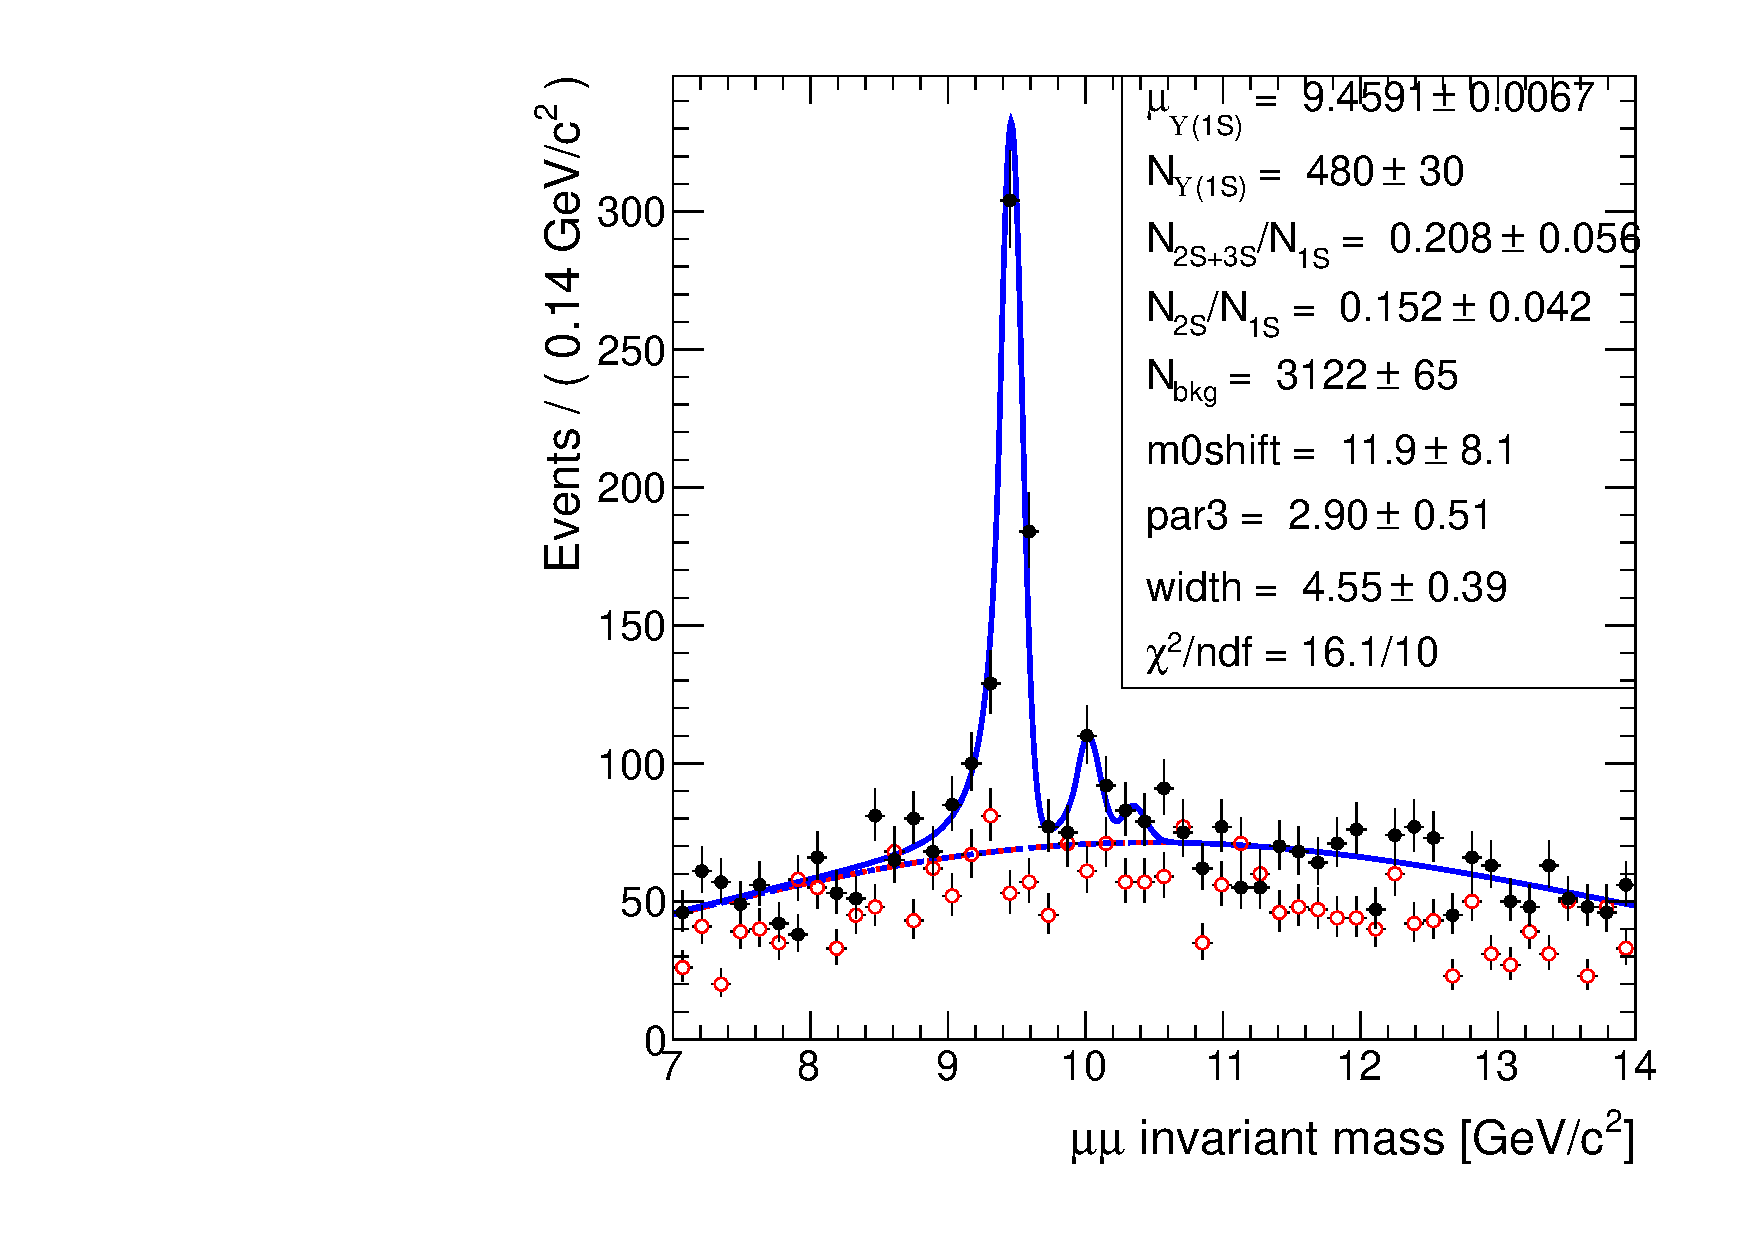
\includegraphics[angle=0,width=0.45\textwidth]{figures/centrality/masspeak_Hi_paramOn_cntr20-50_pt4_150imub}}
%\subfigure[50-100\%]{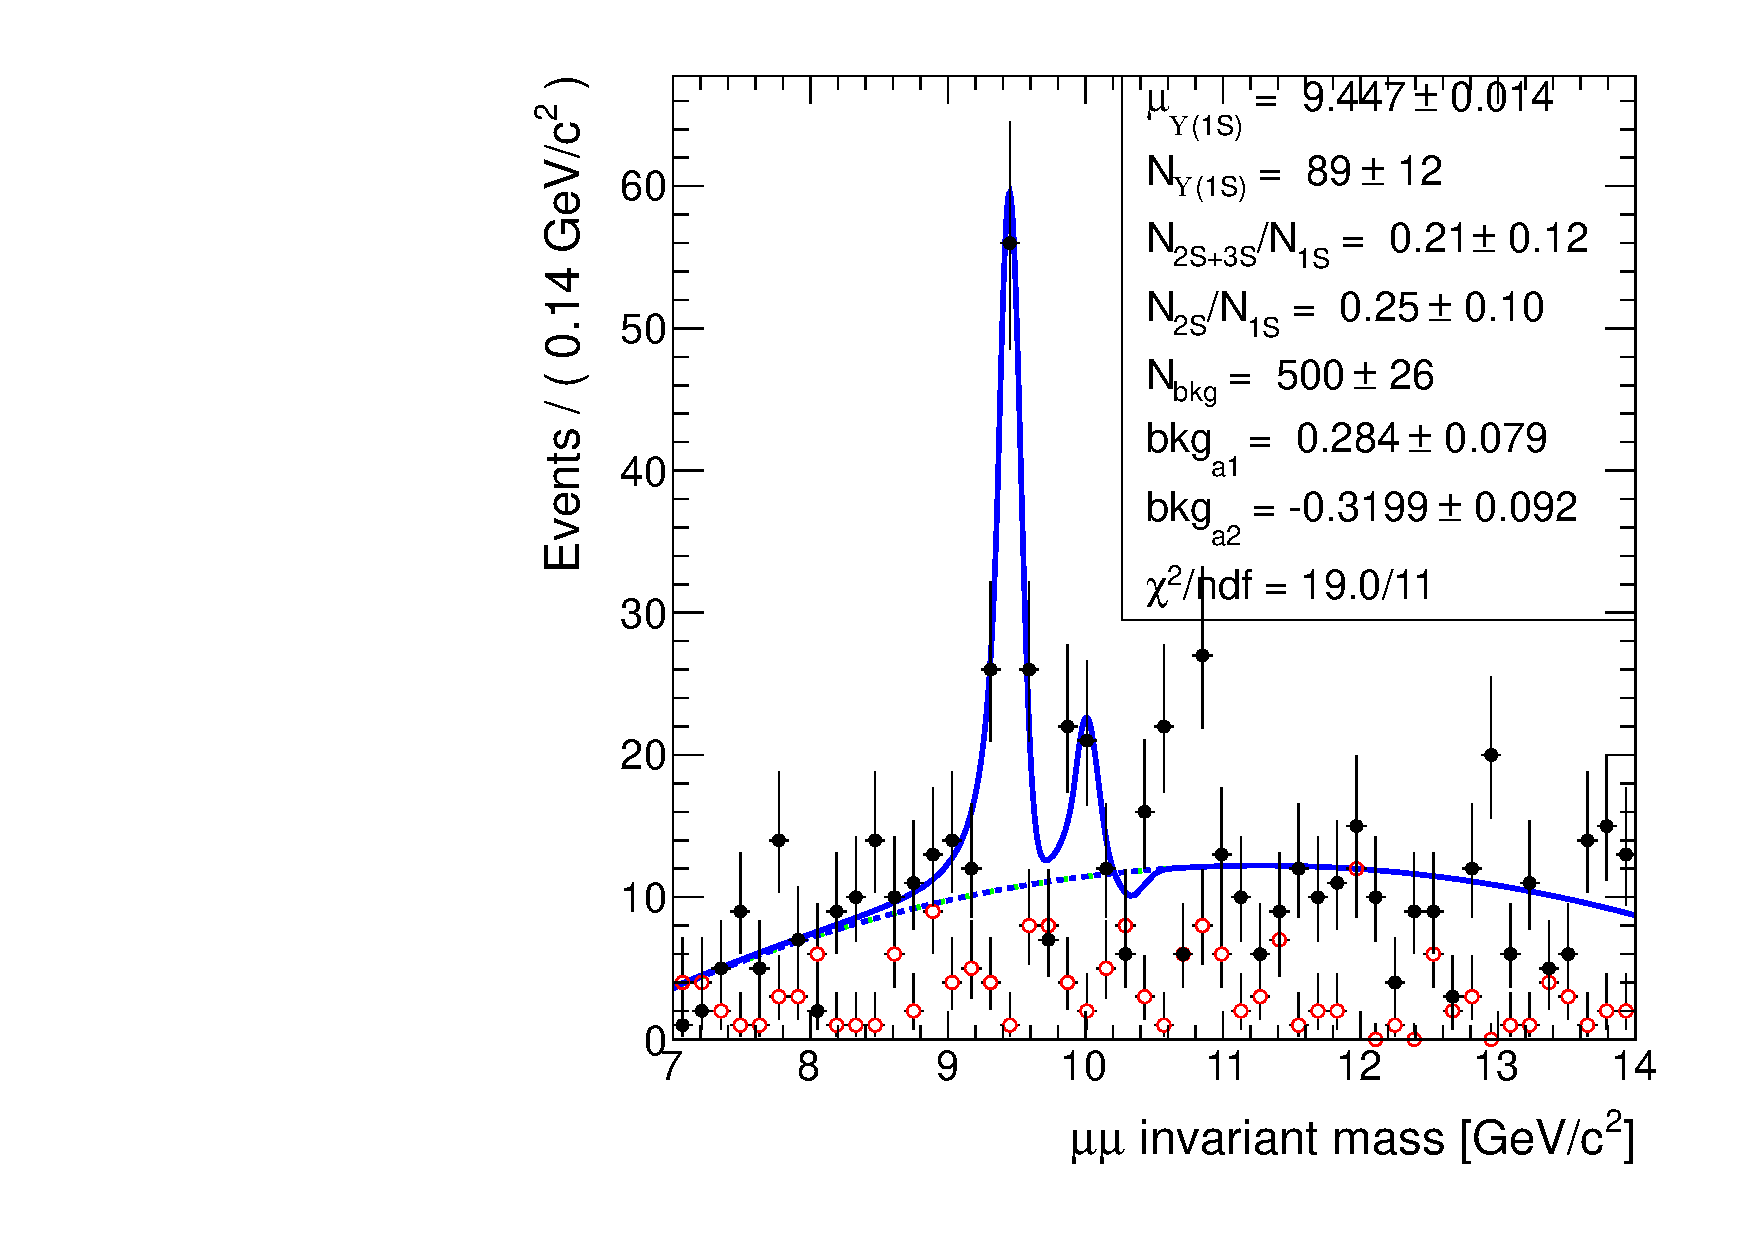
\includegraphics[angle=0,width=0.45\textwidth]{figures/centrality/masspeak_Hi_paramOn_cntr50-100_pt4_150imub}}\\
%\subfigure[Double ratio $\chi_{2}$ vs centrality]{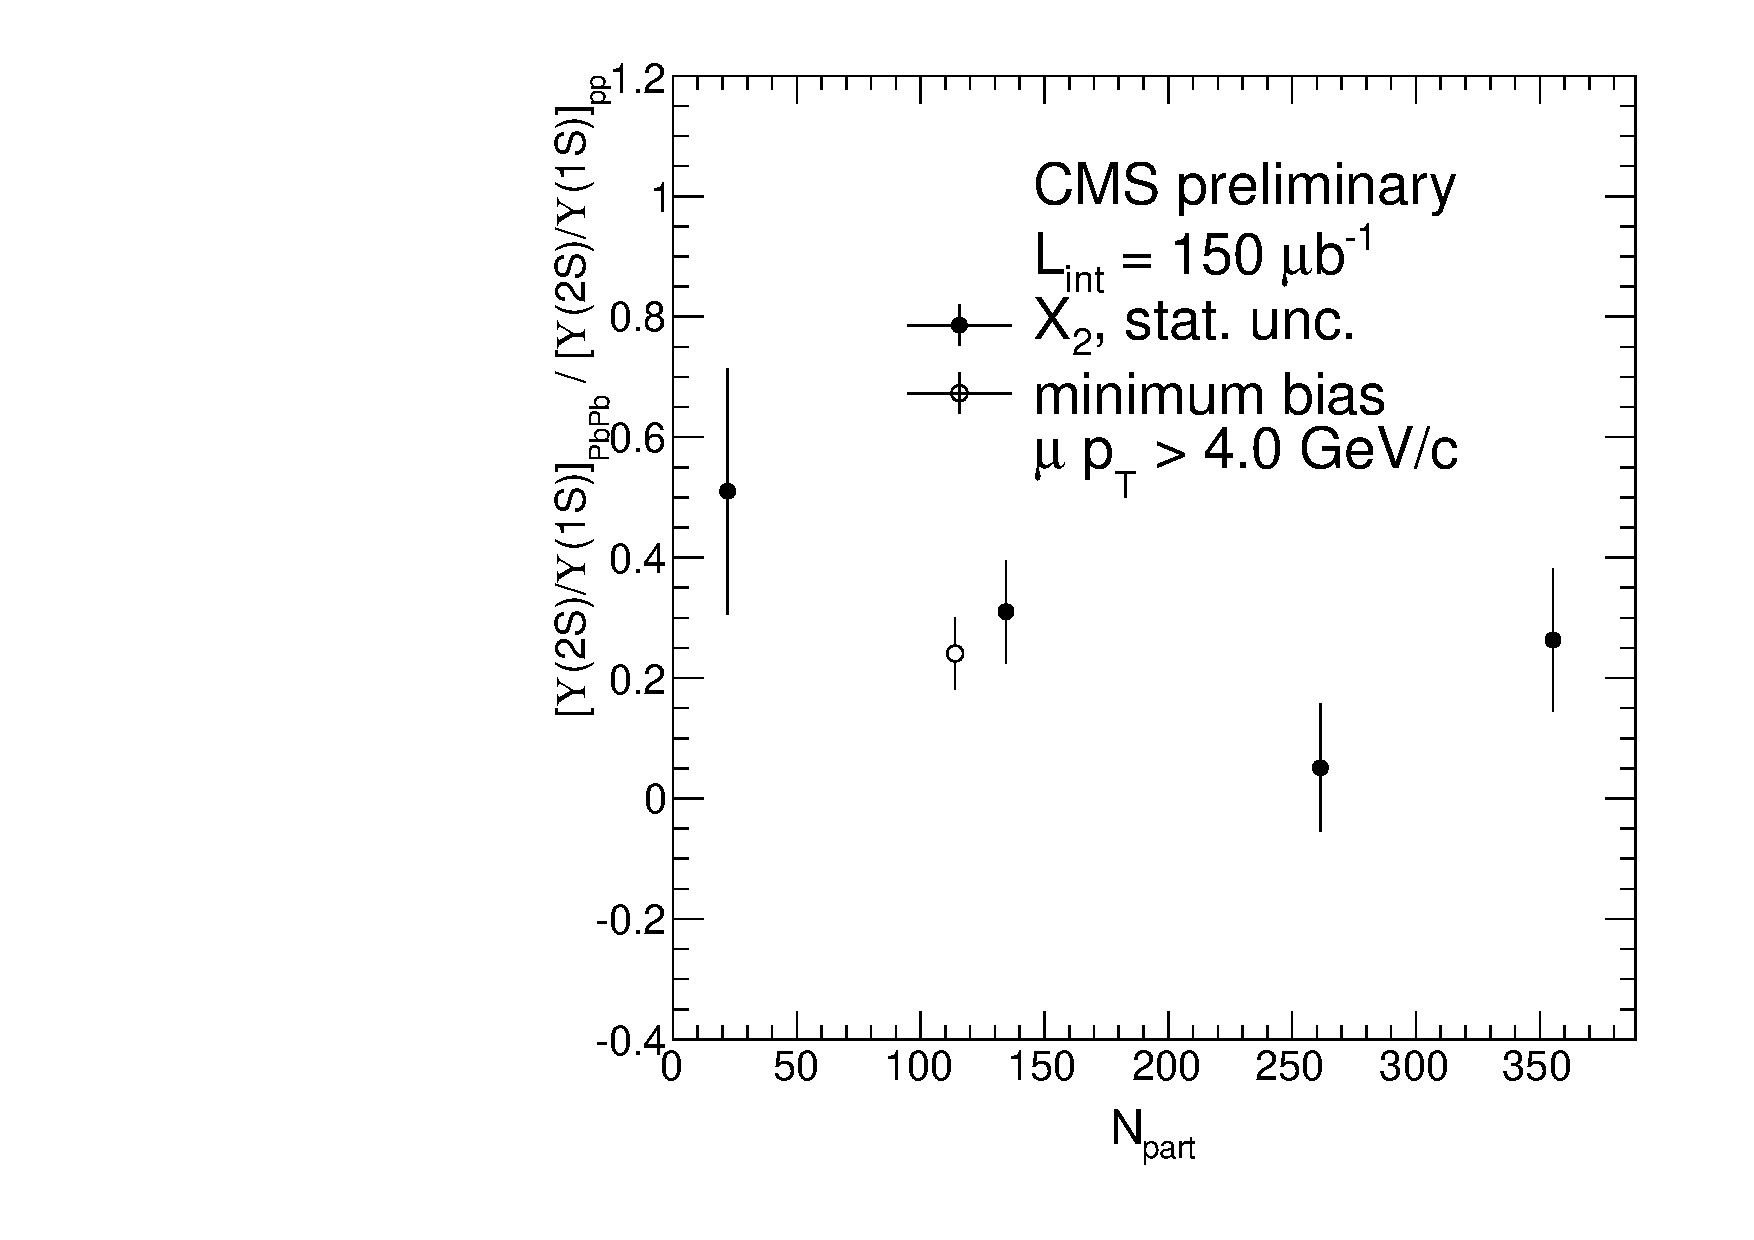
\includegraphics[angle=0,width=0.45\textwidth]{figures/centrality/chi2pt4}} 
%\subfigure[Double ratio $\chi_{23}$ vs centrality]{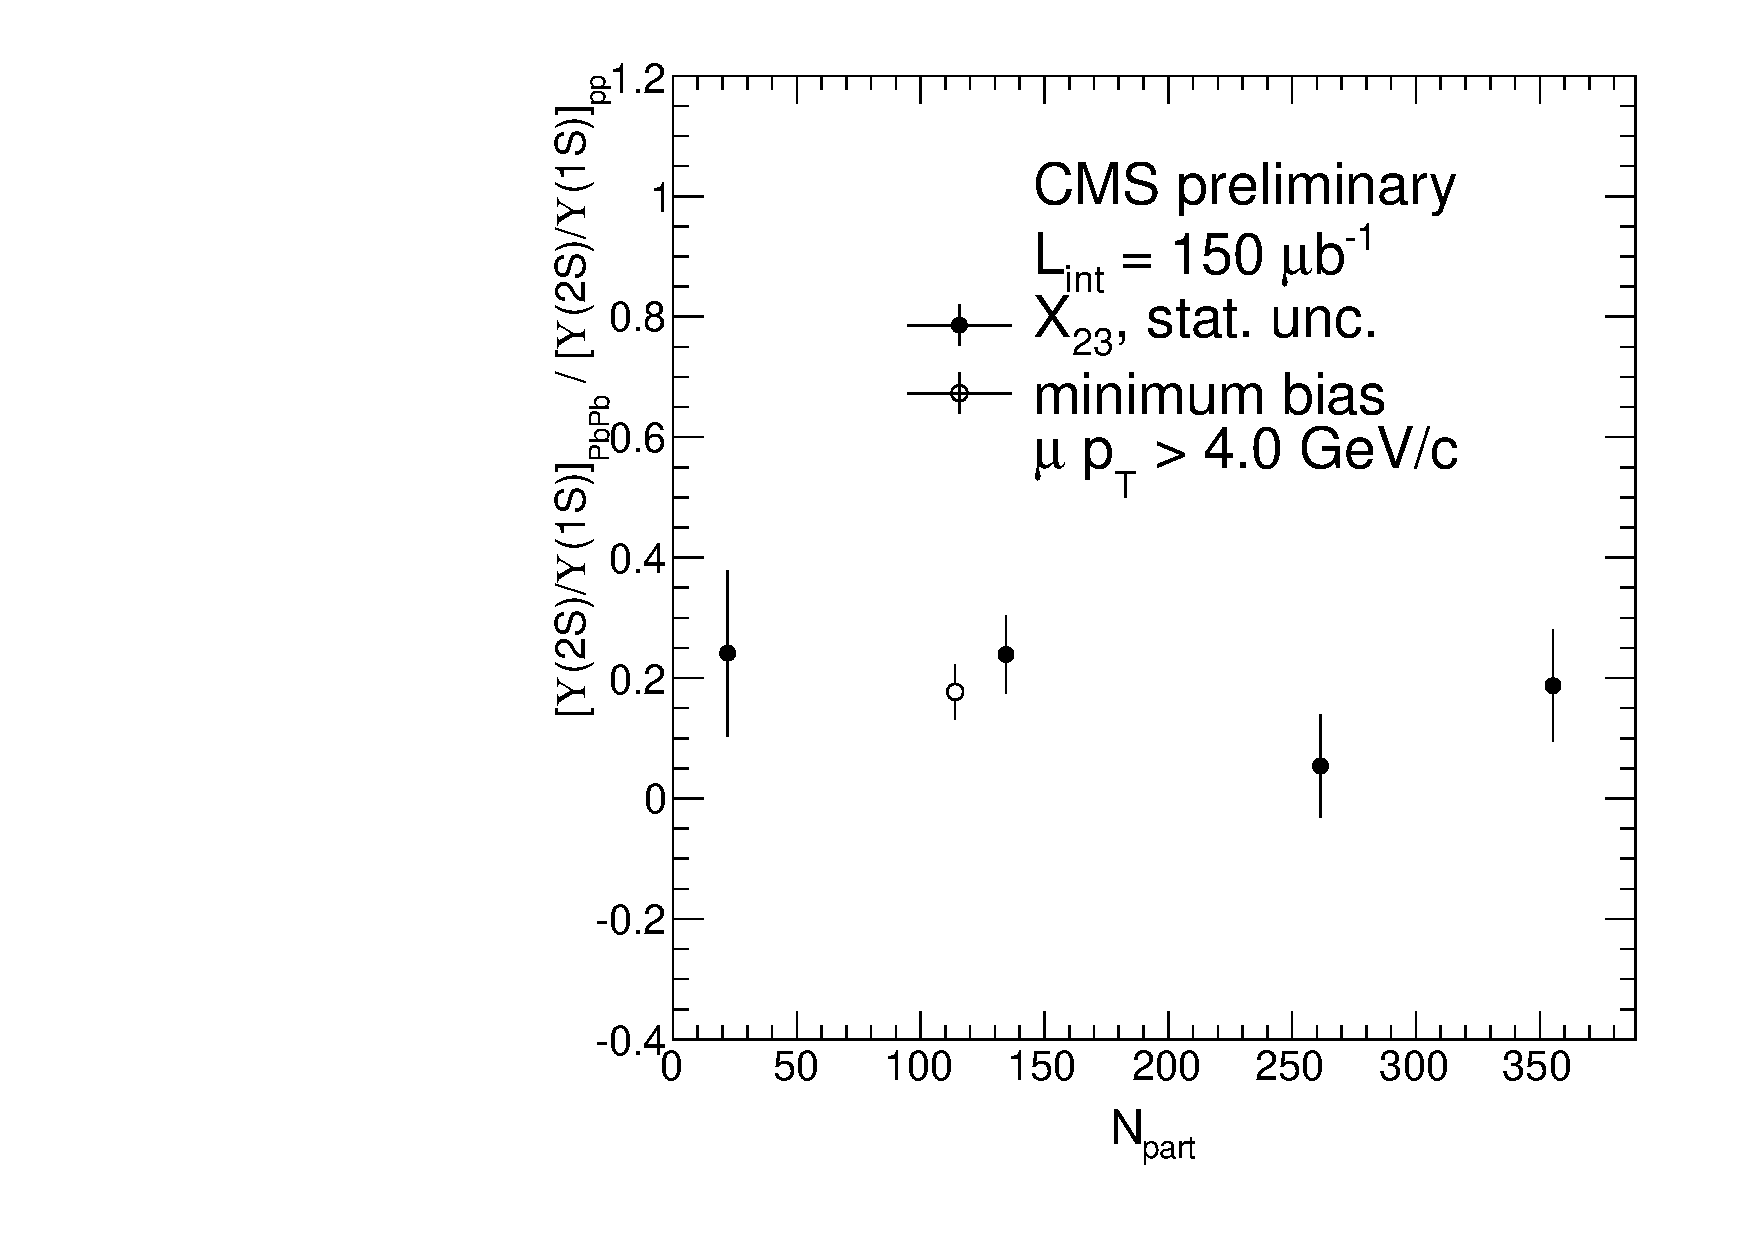
\includegraphics[angle=0,width=0.45\textwidth]{figures/centrality/chi23pt4}} 
%  \caption{Centrality dependent results from the $150 \mu b^{-1}$ dataset. ($\pt>4.0\GeVc$)}
%  \label{fig:massfit_singlerat_centrality_150imub}
%  \end{center}
%\end{figure}

\vskip 1cm 

{\bf{
Latest and older analysis results are thoroughly documented in Ref.~\cite{site-fit}: \\

\hspace{3cm} \href{http://cern.ch/cms-hin-upsilon/fitting}{\sc\large cern.ch/cms-hin-upsilon}
}}